% !TeX program = pdflatex
% !TeX encoding = UTF-8
% !TeX spellcheck = en-US
% !BIB program = bibtex

\documentclass[11pt,a4,oneside,onecolumn,titlepage]{article}

\usepackage{hyperref}

\usepackage{setspace}
\usepackage{geometry}
\geometry{
	%showframe,
	a4paper,
	top=3cm,
	bottom=3cm,
	innermargin=3.9cm,
	outermargin=3.9cm,
}
\usepackage{multicol}
\usepackage{setspace}
\usepackage[utf8]{inputenc}
\usepackage[T1]{fontenc}
\usepackage[]{microtype}

\usepackage[authoryear, round, sort]{natbib}
\let\cite\citep

% colors
\usepackage{color,graphicx}
\usepackage[usenames,dvipsnames]{xcolor}
\usepackage{titlepic}

% math
\usepackage{mathtools} % redefine operators
\usepackage{amssymb}   % needed for mathbb
\usepackage{amsfonts}  % needed for mathbb
\usepackage{mathrsfs}  % needed for mathscr
\usepackage[group-separator={,}, detect-weight=true, detect-family=true]{siunitx}   % replace sistyle, siunits, units
\usepackage{tabu,booktabs,tabularx} % tables
\usepackage{csquotes} % quotes
\usepackage{textcase}
\usepackage[explicit,pagestyles]{titlesec}
\usepackage{parskip} % no parident
\usepackage{xparse}
\usepackage{subcaption}
%\usepackage{showframe}
\usepackage{xfrac}

% font
\renewcommand{\rmdefault}{ppl} % rm
\linespread{1.025}        % Palatino needs more leading
\usepackage[T1]{fontenc}

% checkmark
\usepackage{pifont}%
\newcommand{\cmark}{\ding{51}}%
\newcommand{\xmark}{\ding{55}}%

% Theorems:
\makeatletter



\DeclareRobustCommand{\spacedallcaps}[1]{\sffamily{\MakeTextUppercase{#1}}}%
%\DeclareRobustCommand{\spacedallcapssmall}[1]{\sansbold{\MakeTextUppercase{#1}}}%
\DeclareRobustCommand{\spacedallcapssmall}[1]{{\MakeTextUppercase{#1}}}%
\DeclareRobustCommand{\spacedlowsmallcaps}[1]{\sffamily{\scshape\MakeTextLowercase{#1}}}%


\titleformat{\section}{\raggedright\normalfont\Large\sffamily}{\thesection}{.5em}{{#1}}
\titleformat{\subsection}{\raggedright\normalfont\large\sffamily}{\thesubsection}{1em}{\spacedallcaps{#1}}
\titleformat{\subsubsection}{\normalfont\sffamily}{\thesubsubsection}{1em}{\spacedallcaps{#1}}
\titleformat{\paragraph}{\normalfont\normalsize\sffamily}{\textsc{\MakeTextLowercase{\theparagraph}}}{0pt}{\spacedlowsmallcaps{#1}} 

% graphics
\graphicspath{{./fig/}}


% tables
\renewcommand{\arraystretch}{1.3}
\newcommand{\ra}[1]{\renewcommand{\arraystretch}{#1}}
\newcommand{\maxf}[1]{{\underline{#1}}}

%==============================================
% references
%==============================================
\definecolor{webgreen}           {rgb}{0   ,.5   ,0    }
\definecolor{webbrown}           {rgb}{.6  ,0    ,0    }
\hypersetup{%
	colorlinks=true, 
	urlcolor=black, linkcolor=black, citecolor=blue
}

\DeclarePairedDelimiterX\SetDefX[1]{\lbrace}{\rbrace}{
	\renewcommand\given{  \nonscript\:
		\delimsize\vert
		\nonscript\:
		\mathopen{}
		\allowbreak}
	#1
}
\newcommand\SetDef{\SetDefX}

% conditional distribution
\DeclarePairedDelimiterX\conditionX[1]{}{}{
	\renewcommand\given{  \nonscript\:
		\delimsize\vert
		\nonscript\:
		\mathopen{}
		\allowbreak}
	#1
}
\newcommand\condition{\conditionX}

\widowpenalty10000
\clubpenalty10000

\usepackage{tcolorbox}

\begin{document}

%% Front page of thesis
	\title{\normalfont\spacedallcaps{Anomaly Detection in the time series data of motor vibrations}}
	\author{\spacedlowsmallcaps{Samuel Bancroft, Alexander Bell, Danielle Eden,}\\
		\spacedlowsmallcaps{Jake Farr, Robert Mercer \& Teodor Tzokov}
		\\ {\textit{Department of Physics, Durham University}}}
	\date{\today}
	\titlepic{
\includegraphics[width=0.3\textwidth]{formatting/DU_2-col_sml.eps}}
\maketitle
	
\begin{center}
	\begin{tcolorbox}[colback=white,width=\textwidth,colframe=white]
		\section*{\large Abstract}
		\small
		Outline, Methods, Outcomes, Conclusions. ABSTRACT GOES HERE
	\end{tcolorbox}
\end{center}
		
\newpage

\tableofcontents
\clearpage
\listoffigures
\listoftables
\clearpage


%% Main text
% set page number starts from 1
\pagenumbering{arabic}
\setcounter{page}{1}

\section{Introduction}
\label{sec:introduction}

\subsection{Anomaly Detection}
\label{subsec:anomaly_detection}

\begin{figure}[t]
    \centering
    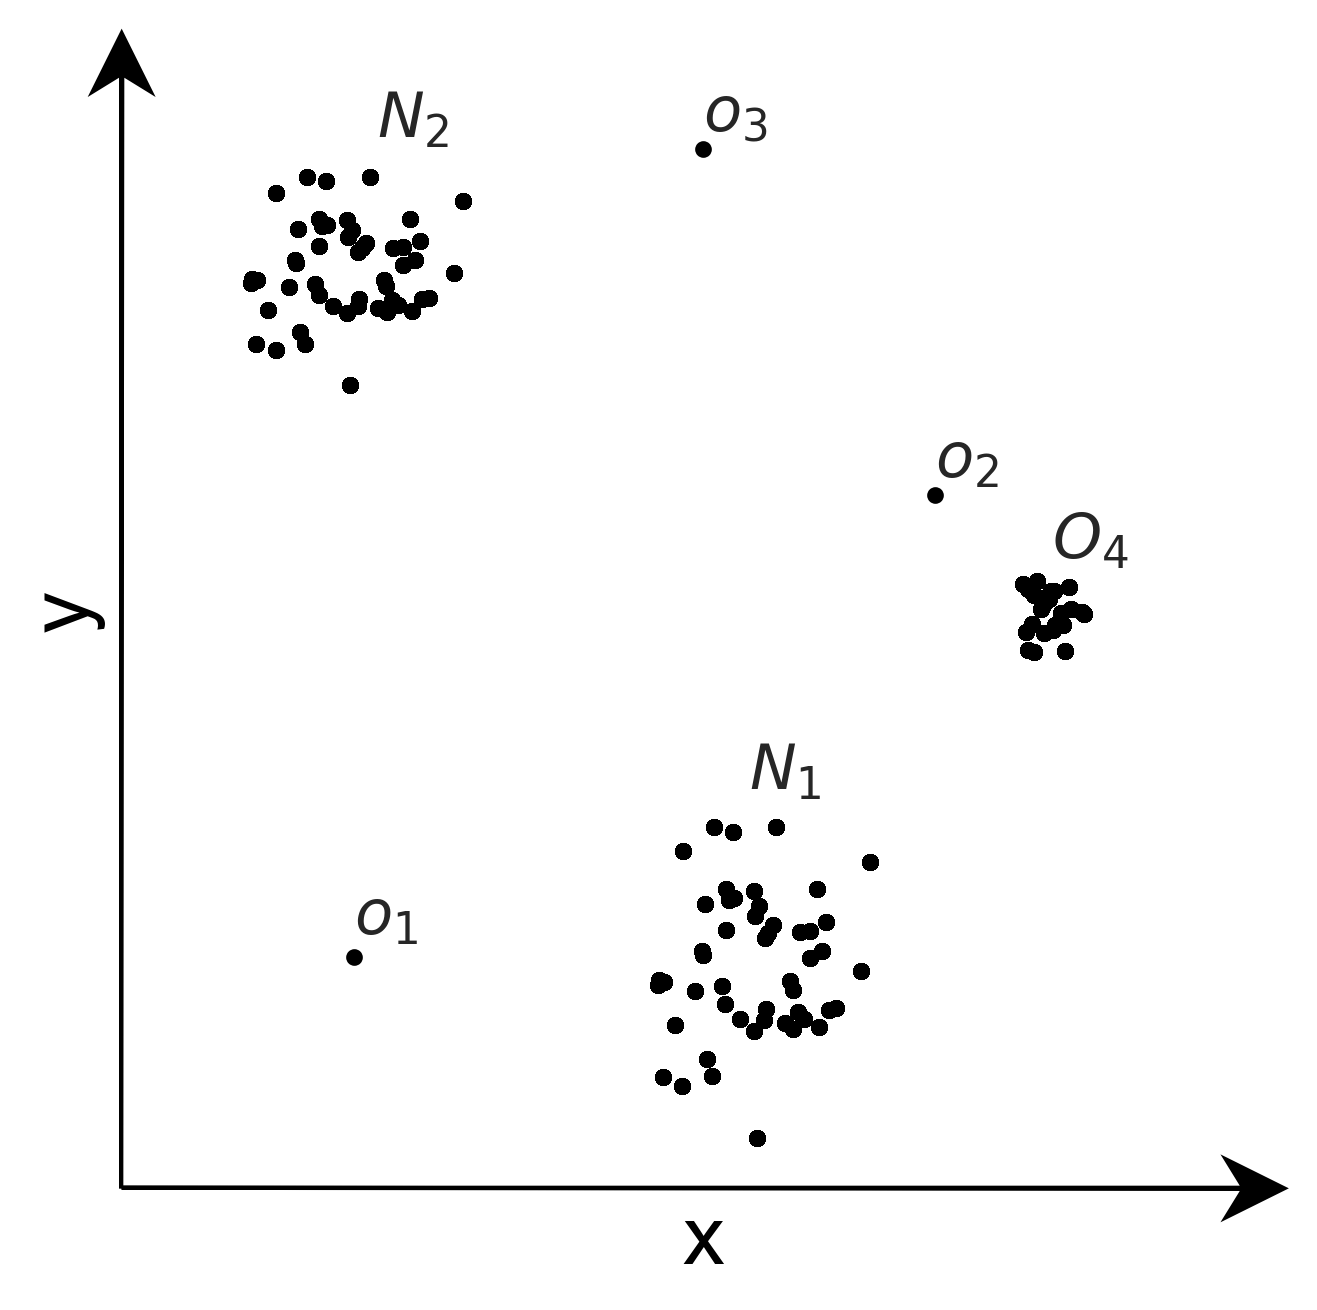
\includegraphics[width=0.6\textwidth]{fig/anomalies.png}
    \caption[Example of Anomalies]{A simple example of a 2D data set containing anomalies, where $N_{1}$ and $N_{2}$ are the `normal' data points and the surrounding points are anomalous.}
    \label{fig:anomalies}
\end{figure}

An anomaly is defined as a data point that does not conform to the expectations of a system, as illustrated in Figure.~\ref{fig:anomalies}. In this example, there are two regions containing normally distributed data, $N_{1}$ and $N_{2}$, where the majority of the data points are concentrated. The surrounding points, $O_{1}$ through to $O_{4}$, are a sufficient distance from the normal data that they are classed as anomalous. Anomaly detection is the process of finding these anomalous data points \cite{huang}. This information can be extremely important and can be applied in a range of ways in order to find out more from a data set. The way in which data is anomalous can also be indicative of what could be the cause, as two different issues could lead to anomalies, and present themselves in different ways. 

The detection of anomalies is crucial both in data cleaning processes, and in the detection of any upcoming issues when monitoring live data \cite{Akouemo2016948}. This has many important real world applications, including those in cyber-security and finance in detecting fraudulent behaviours automatically \cite{618940}. Anomaly detection works under the assumption that a dataset will contain a large number of `normal' points and a few `abnormal' points, taken as the anomalies \cite{Pimentel2014215}. In the scope of this project, anomalies will be produced by unusual behaviour from the motor: caused by issues such as overheating, components beginning to break, or overloading the motor and applying more stress than it can take. 

Anomaly detection has a wide range of real world applications, all of which are crucial when finding issues with equipment in real time or suspicious behaviour in certain data types. Some examples being in credit card fraud detection, medical diagnosis and failure detection in industrial environments. It was first introduced in 1987 for Intrusion Detection Systems (IDS) by Denning for online security, which worked on the assumption that the exploitation of a system's weaknesses would involve abnormal behaviour \cite{1702202}. 

Since this initial application, the use of anomaly detection in cyber-security has become standard, and is crucial for uses such as detecting fraudulent credit card transactions or suspicious online traffic patterns. Before this, one of the first applications of anomaly detection were the Western Electric Rules, which were a set of decision rules that were used to determine `out of control' data (Western Electric Co., \citeyear{statistical_quality_control_handbook_1956}). This was decided by the number of points that were a certain number of standard deviations from the centreline. For example, a single point more than three standard deviations from the centreline or two out of three consecutive points more than two standard deviations away were deemed unstable. These four rules were used to determine when data was beginning to behave in an unpredictable manner. 

Nowadays, anomaly detection has uses in a wide range of fields, including the medical field: Computer Aided Diagnosis (CAD) is used alongside professionals to improve the rates of false positives or undetected anomalies. An anomaly in a mammogram could be an indication of a tumour for example \cite{Sajda2003AMP}. Spacecraft can be monitored using anomaly detection methods to ensure that any failures in equipment are detected early, when the spacecraft is in use and cannot be observed in person \cite{Fujimaki:2005:ADM:2140831.2140938}. Clearly, anomaly detection is a wide ranging field, which has a number of applications in different areas, most of which are extremely important and lead to actionable results.

There are five distinct ways in which anomaly detection can be carried out: probabilistic, distance-based, reconstruction-based, domain-based and information-theoretic based \cite{Pimentel2014215}. The probabilistic approach will estimate the characteristics of a dataset based on the density of points in a `normal' set and compare data to this set to determine which points are anomalous based on the probability of a point being in that position. The distance-based approach assumes that `normal' data will be tightly clustered, and anomalous points will be a distance from these points. Clustering analysis or nearest neighbour analysis is then used to determine whether or not a point is anomalous. Reconstruction-based analysis involves using a training set of data and mapping data using the model that has been created. A large difference between the model and the observed data will result in a high anomaly score, and hence the point will be deemed anomalous. The domain-based approach produces a boundary surrounding the `normal' data, and determines that any point outside of this is anomalous. Finally, using the information-theoretic approach, measures such as entropy are calculated, and it is assumed that anomalous data will significantly change the value of this. A combination of methods will be used to determine where anomalies are found in order to improve the reliability of detecting anomalous points and minimise the chance of false positives.

In our project, anomaly detection has been applied to the vibrations measured on an electric motor whilst running. All electric motors generate vibrations as they move. Analysis of vibration data can be used be used to diagnose the health and general performance of a machine \cite{DelgadoArredondo2017568}. Vibrations in electric motors are caused by forces that are all of a magnetic, mechanical or aerodynamic nature \cite{dorrell_smith_1996}. Various faults and asymmetries have been well identified through vibration signal diagnostics. Typical faults that manifest their signatures in vibration signals include rotor asymmetries, gear faults, unbalanced rotors and faults in the motor bearings. Throughout this project, the vibrations of motors will be monitored, and analysis on this data will allow for the detection of faults. Doing this with live data could mean that faults are detected as they begin, alerting the user and allowing for action before the fault becomes significantly problematic to the system.

Some previous research has been done into vibrational analysis of motors to detect failures. Most examples of this use a distance-based approach or a reconstruction-based approach. In particular, a health index called the Mahalanobis distance has been used as a distance-based approach \cite{Jin20135787} and machine learning has been applied as a reconstruction-based approach \cite{5899067}.

The vibrations from the motor that are being monitored are classed as a continuous signal, as they are taken after equally spaced amounts of time over a given period. This means the data can be defined as time series data, which is simply a series of data points that are taken in chronological order in equally spaced chunks. For scalars this is defined as:

\begin{equation}
    \{x(t_0), x(t_1), ..., x(t_{i-1}), x(t_i), x(t_{i+1}), ...\}~.
\end{equation}

The vibrations of electric motors can be defined as a continuous signal $x(t)$ where $t$ is real-valued. In order to obtain a sample $\{x[t]\}$ one must uniformly sample the signal at discrete points. For a sampling period of $\Delta t$, the obtained sample is defined as,

\begin{equation}
    \{x[t]\} = \{x(0), x(\Delta t), x(2\Delta t), x(3\Delta t),...\}~.
\end{equation}

To recover $x(t)$ from $x[t]$, there must be an appropriate choice for the value of $\Delta t$ in accordance with the Nyquist–Shannon Sampling Theorem. This theorem states that a sampling frequency must be at least twice as high as the highest frequency component of $x(t)$. If not, an aliasing of frequencies will become apparent \cite{Ficker2015}. It is for this reason that 3000 Hz was chosen as the sampling frequency; it is more than double any frequency we expect to measure.

The motivation for this project has been to investigate how motors act when they begin to experience a fault in order to recognise issues in the future. Knowing the way in which a motor behaves when it begins to malfunction could mean motors can be monitored in real time and faults detected as they begin. This could lead to the prevention of some motors malfunctioning completely if the problem is caught early on.

\clearpage
\subsection{Structure of Report}

In \S\ref{sec:methods} we describe the various anomaly detection methods that we have developed and how they have been created and work. We include a discussion about anomaly detection in both the time domain, and frequency space. A range of approaches are covered, with their positive and negative aspects discussed. Methods that were subsequently rejected have also been mentioned.

In \S\ref{sec:analysis} we examine each motor failure mode that was investigated. The theory behind each failure mode is discussed, as well as the method that we took in order to induce that kind of failure. We then consider the limitations and relative performance of various anomaly detection methods and their various successes at diagnosing particular kinds of motor anomalies.

In \S\ref{sec:conclusion} we discuss the future of anomaly detection, and offer suggestions for future development in the detection of motor anomalies from their vibration signals. The specific methods that we find the most suitable are discussed, as well as the best way to implement the anomaly detection as a whole. We conclude with our final remarks.      %EVERYONE
\section{Anomaly Detection Methods}
\label{sec:methods}

As part of the data reduction procedure, a moving average was applied to data in both the time domain and the frequency domain. A moving average essentially applies a low-pass filter to the data.

For the time domain, this was mainly applied in order to ensure more accurate reconstructions when using techniques such as K-mean Clustering Reconstruction (see \S~\ref{subsec:kmeans}) and LSTM Recurrent Neural Networks (see \S~\ref{subsec:LSTM}).

For the frequency domain, the moving average was applied to the frequency domain, after the Fourier transform has already been applied to the unaltered time series data. This ensures that all of the higher frequencies were not lost.

The method of taking a moving average is implemented using the convolution of the data with a kernel, $k$. If a moving average with width $w$ is required, the kernel is defined as,

\begin{equation}
    k = \left[ \dfrac{1}{w}~\dfrac{1}{w}~\dfrac{1}{w}...\dfrac{1}{w}  \right]~,
    \label{eq:conv_kernel}
\end{equation}

where the array is of length $w$. This is then convolved with the data set, which has the effect of `smoothing' the data.

\begin{figure}[t]
    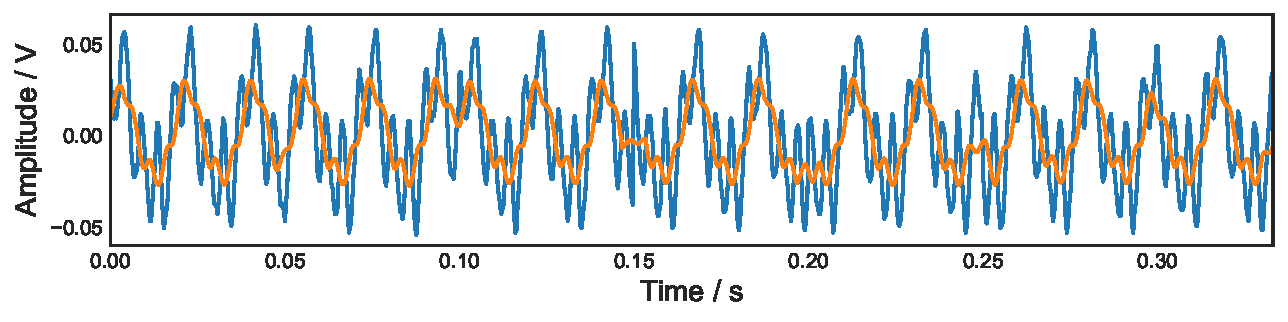
\includegraphics[width=1.0\textwidth]{fig/moving_average.pdf}
    \caption[Time Domain]{Moving average applied to data in the time domain. The original data (shown in blue) represents the amplitude of the signal as a function of time. The orange curve shows the moving average of this data.}
    \label{fig:moving_av}
\end{figure}

\begin{figure}[t]
    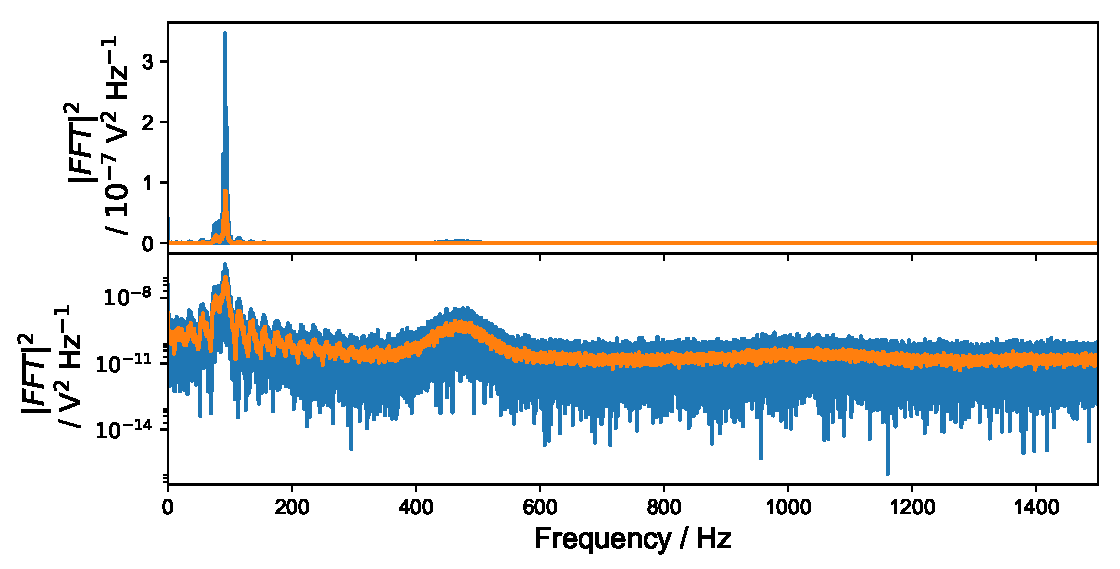
\includegraphics[width=1.0\textwidth]{fig/freq_moving_average.pdf}
    \caption[Moving Average in Fourier Domain]{Moving average applied to data in the Fourier domain, shown in both linear and logarithmic axes. The blue lines show the original amplitudes as a function of frequency. The orange lines show the moving averages.}
    \label{fig:freq_moving_av}
\end{figure}

Figures.~\ref{fig:moving_av} and ~\ref{fig:freq_moving_av} show examples of applying a moving average to data in the time domain and frequency domain, respectively. 


----Moving average for dealing with issues with the resloution for the raw data in the y axis

\subsection{Statistical Approach}

The most simple methods for detecting changes from `normal' motor behaviour can either use simple value thresholds, or static mean and standard deviation calculates to determine when data experiences a significant deviation from usual patterns. 

Such basic approaches are not easily adapted for use in time series data. This is because:

\begin{enumerate}
    \item These methods are not easily applied to changing data values.
    \item They cannot scale easily to large time series.
    \item An unacceptable quantity of false anomalies can be detected.
    \item They rely on the assumption of a normal distribution of data points, which is not always the case for time series data.
\end{enumerate}

Nevertheless, these approaches can provide immediate indications of the most obvious anomalies. 

In order to ensure that the data the statistical tests were applied to followed a Gaussian distribution, a moving average was first taken.

\begin{figure}[t]
    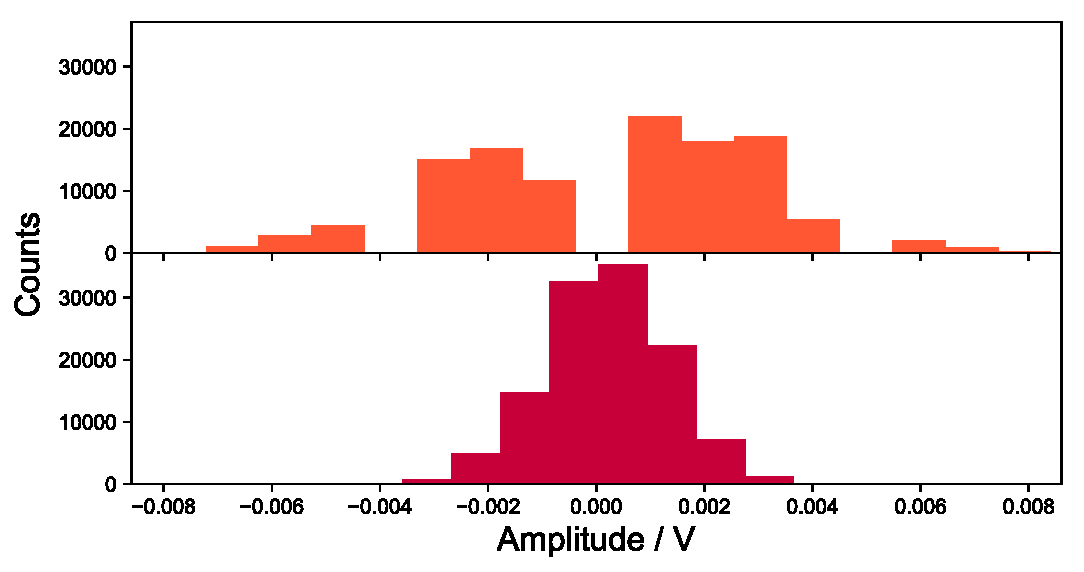
\includegraphics[width=1.0\textwidth]{fig/moving_av_hist.pdf}
    \caption[Moving Average Histogram]{Histograms for the raw data (top) and when a moving average with a window size of $w=20$ is applied (bottom).}
    \label{fig:move_av_hist}
\end{figure}

Figure.~\ref{fig:move_av_hist} shows how the distribution for the moving-averaged data has a Gaussian distribution, whereas the raw data does not.

It was therefore necessary to apply a moving average to the raw data before any statistical tests were performed.

\subsubsection{Histogram Test}

\begin{figure}[t]
    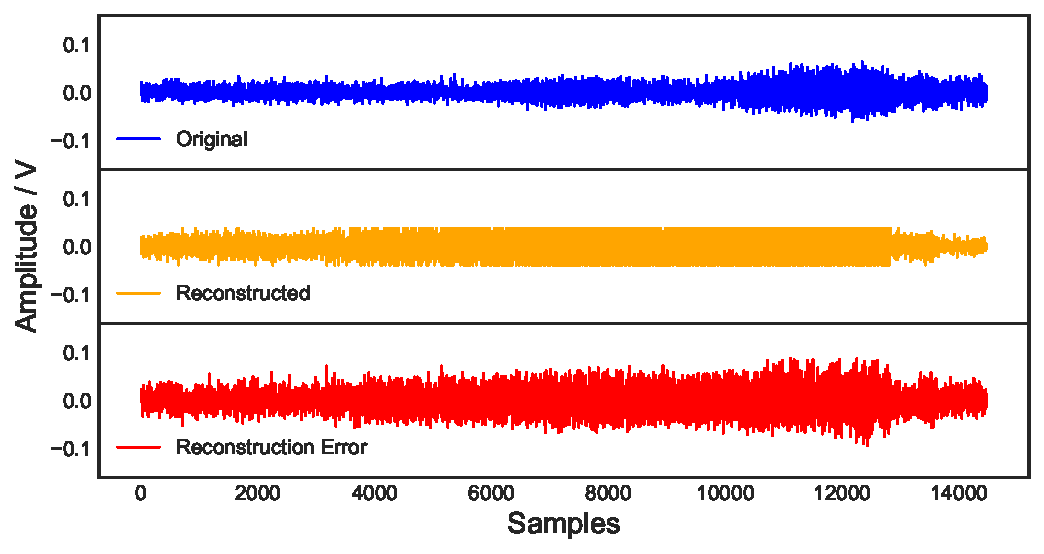
\includegraphics[width=1.0\textwidth]{fig/histogram.pdf}
    \caption[Histogram]{Histogram method}
    \label{fig:histogram}
\end{figure}

The histogram test first assumes that the recorded data is normally distributed, so that the probability $p$ of a value $x$ is,

\begin{equation}
    p(x) = \dfrac{1}{\sigma \sqrt{2\pi}}\exp(\dfrac{-{(x-\mu)}^2}{2\sigma^2})~,
\end{equation}

where $\mu$ and $\sigma$ are the mean and standard deviation of the sample respectively.

The method begins by separating the a `training' time series sample into equal bins. This training sample serves as a set of example data that represents the expected behaviour. The median value of each of these bins is then calculated.

A reconstruction of a time series is then carried out. For each value in the time series, the difference between the defined medians, and the value is calculated. The smallest difference is then chosen to represent the reconstruction of the time series.

Figure.~\ref{fig:histogram} shows an example of the histogram method for an arbitrary time series. The reconstruction error represents the difference between the original time series and the reconstructed time series. The training data was taken from a motor operating at the same voltage as the test data, under normal baseline conditions.

\subsubsection{Grubbs' Test}
One of the most commonly used statistical threshold tests for outliers is the two-sided Grubbs' Test \cite{CIS-320511}.

For the two-sided Grubbs' test, this involves defining a Grubbs' test statistic as,

\begin{equation}
    G = \dfrac{\underset{i=1,2,...,N}{\max}|\mathcal{X}_i-\bar{\mathcal{X}}|}{\sigma}~,
    \label{eq:grubbs}
\end{equation}

where $\mathcal{X}$ denotes a set of data of length $N$, and $\bar{\mathcal{X}}$ and $\sigma$ are the mean and standard deviation of this data set, respectively. $G$ is equivalent to the largest deviation from the mean in units of standard deviations.  

The hypothesis of no outliers being present is rejected if,

\begin{equation}
    G > \dfrac{N-1}{\sqrt{N}} \sqrt{\dfrac{(t_{\alpha/(2N), N-2})^2}{N-2+(t_{\alpha/(2N), N-2})^2}} ~,
    \label{grubbs_condition}
\end{equation}

where $t_{\alpha/(2N), N-2}$ denotes the $t$-distribution with a significant level of $\alpha/(2N)$ and $(N-2)$ degrees of freedom. 

The Grubbs' test is useful in identifying if an outlier exists in the data set, however it is very limited. It only identifies if the data is anomalous, and does not indicate how many anomalies there are or indicate where in time the anomalies are.

Nevertheless, it can be used as a very quick indication of whether results are anomalous in amplitude over time. If it indicates outliers are present, more rigorous statistical tests can be used to determined where and when outlier occurred. 

\subsubsection{Standard Deviation Test}
Assuming that a data set is normally distributed, a simple threshold test on the residuals from the mean can be used to detect outliers. 
Although a deviation of more than $3\sigma$ can in some cases be considered to be anomalous, there is still a $0.3\%$ chance of a data point following the normal distribution to fall more than $3\sigma$ from the mean. In some cases, the data sets analysed in this report can exceed $100,000$ entries. Using a $3\sigma$ threshold test in this case would lead to $300$ false positives. Alternatively, with a sampling rate of $3000$ Hz, this would equate to $9$ incorrect outlier alerts every second. 

Instead, $5\sigma$ was used as the threshold for the residuals. The likelihood of a normal data point deviating from the mean by more than $5\sigma$ is $3 \times 10^{-7}$, giving a much lower false positive detection rate of one every $\sim 18$ minutes. 

Therefore for the purpose of this report, a data point deviating by more than $5\sigma$ from the mean is considered to be an anomaly. 

This method can be used to find multiple anomalies within a data set, with their respective positions in time.

\subsubsection{Deviation From Moving Average}
This is a similar method to the standard deviation test, but instead of calculating the mean and standard deviation of the entire sample, a moving mean and standard deviation are taken. A window size of 50 for the moving average was used.
If a data point deviates from the moving average by 4 moving standard deviations or more, then it is considered to be an outlier. This method is better for detecting just the anomalies at shorter time scales, whereas the Standard Deviation Test detects both short scale and more gradual amplitude changes. 

Unlike the previous two tests, this is applied to the raw data, as the test itself involves smoothing the data and comparing this to the raw data.


\subsection{Fourier Analysis}

\begin{figure}[t]
    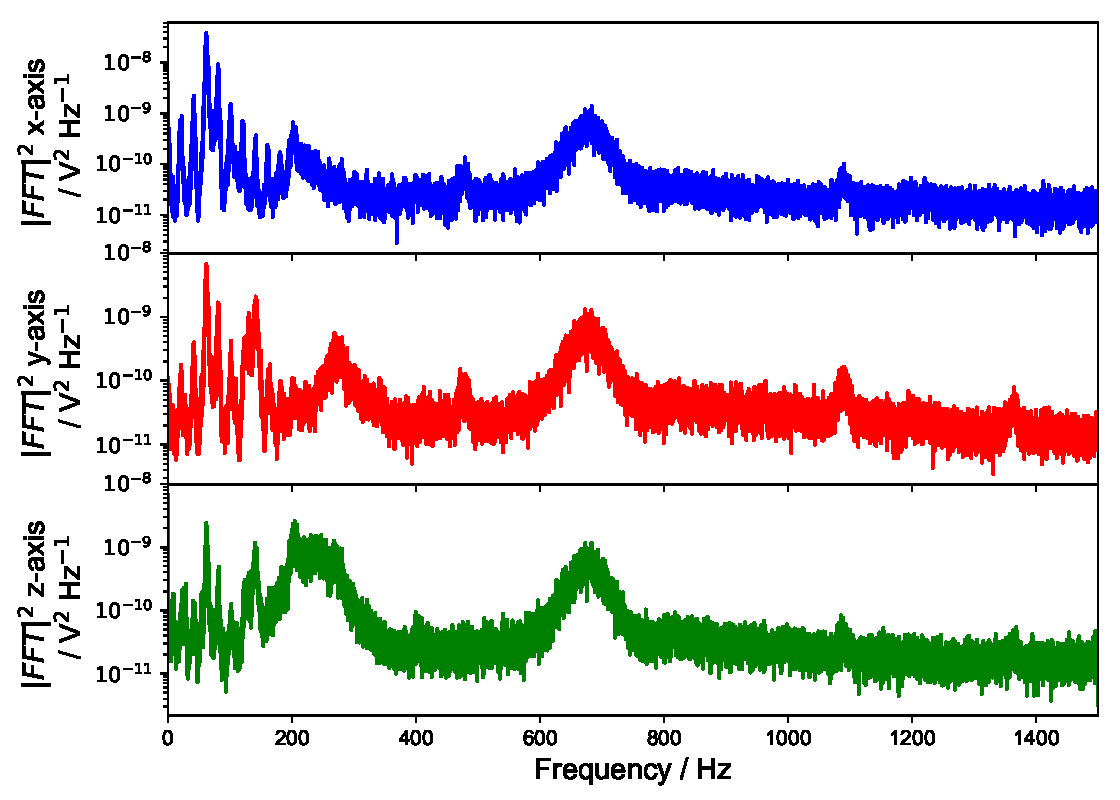
\includegraphics[width=1.0\textwidth]{fig/freq_theory.pdf}
    \caption[Fourier Spectrum of 12 V motor in $xys$ axes]{Amplitudes as a function of frequency for the 12 V motor in all 3 axes. }
    \label{fig:frequencies}
\end{figure}

Fourier transforms of time series data are used to provide a mapping between the time domain and the frequency domain, finding the amplitude of the constituent frequencies \cite{hsu_1984}. Another term for this frequency domain representation is the spectrum of the signal. 

This transformation was implemented using a Fast Fourier Transform (henceforth FFT), in order to perform a discrete fourier transform (DFT). If time series data consists of a set of data of length $N$, $\{ x_0, x_1,...,x_{N-1} \}$, the DFT is defined as \cite{hsu_1984},

\begin{equation}
    y_k = \sum_{m=0}^{N-1} x_m \cdot e^{-2\pi ikm/N} \quad (k = 0,1,...,N-1)~,
    \label{eq:DFT}
\end{equation}

where $y_k$ is the amplitude for a given $k$. $k$ is related to frequency, and the frequency $f$ can be obtained using the equation,

\begin{equation}
    f = \dfrac{k}{N} \times S~,
    \label{eq:freq_from_k}
\end{equation}

where $S$ is the sampling rate with which the data was collected ($S=3000$ Hz for this work). Therefore Eq. \eqref{eq:DFT} returns values of $y_k$, for $k = 0,1,...,N-1$, making $N$ values in total, that correspond to amplitudes for equally spaced frequencies between $0$ and $3000$ Hz. However, due to the Nyquist-Shannon Sampling Theorem (see \S\ref{subsec:anomaly_detection}), only the first half of these frequencies can be properly resolved, and so the second half of the $y_k$ values are discarded.

When representing the spectrum, the power spectral density (PSD) was used, which is found by multiplying the complex amplitude obtained from the $FFT$ by its complex conjugate, giving $|FFT|^2$. This is useful as it is proportional to the power output per unit frequency, and in addition makes peaks more visually prominent in the spectrum. The $|FFT|^2$ was then normalised by dividing by $N$, the length of the data, to ensure the amplitudes of peaks in Fourier space do not depend on the length of data used to generate them (so that a spectrum taken from 2 seconds of data will have the same amplitudes as one taken from 2 minutes of data).

Figure~\ref{fig:frequencies} shows the power spectral density returned using this method. A logarithmic axis is used to make the less prominent peaks visible.

\subsubsection{Gaussian fitting in frequency space}

In addition to visual inspection of the spectra, a more quantitative approach was attempted. This was achieved by fitting a Gaussian curve to the most prominent peak in the spectrum. This was done by varying the parameters of the Gaussian and using a least-squares regression algorithm to minimise the residuals between the data and the Gaussian curve. A Lorentzian curve was also attempted, but the Gaussian generally gave a smaller sum of residuals and so is the method used. 

A Gaussian peak is defined by,

\begin{equation}
   \mathcal{G}(f) = A e^{-(f-\mu)^2/2\sigma^2}~,
    \label{eq:gaussian}
\end{equation}

where $A$ is the amplitude of the Gaussian, equal to the maximum amplitude of the peak; $\sigma$ describes the width of the peak and is related to the full-width at half-maximum (FWHM) by $FHWM = 2\sigma \sqrt{2ln2}$, and $\mu$ is the frequency of the centre of the peak. The total area under the peak is given by $\sqrt{2\pi}\sigma A$.

Time series data from a "healthy" motor (one in which no possible faults have been purposefully imposed) were subdivided into segments and spectra obtained in all three motor axes. These were used to generate a set of Gaussians for the most prominent peak in each, each described by the three parameters $A$, $\sigma$ and $\mu$, defined above.

Initially, baseline data was split into three second segments and a Fourier spectrum was obtained for each segment. A Gaussian curve was fitted to the most prominent peak in each spectrum. This was used to create a database of values for $A$, $\sigma$ and $\mu$ from each segment. From this, a mean and standard deviation (error) was obtained for $A$, $\sigma$ and $\mu$. 

This process was then repeated for data that was recorded when trying to induce failures, in order to again determine values for $A$, $\sigma$ and $\mu$ with their respective errors. If any of $A$, $\sigma$ or $\mu$ do not agree within their errors with the values obtained from the "healthy" baseline data, then there is an indication that the frequency response of the motor is changing. This technique can be very useful in autonomously tracking the frequency response of a motor. As many failure modes can manifest themselves as gradual changes in the frequency of the motor, this technique can be useful for detecting signs of failure that the statistical tests applied to amplitudes in the time domain fail to identify. 
 
\subsubsection{Harmonic Frequencies}


\subsection{Least Squares Anomaly Detection}
Included amongst our anomaly detection methods is a squared-loss objective function which is quick to detect anomalous data given a set of training and testing datasets. Due to the rudimentary nature of the function and the very simple analytical solution it has a speed advantage over other methods, as well as presenting a static anomaly score across the train and test data to visualise the magnitude of the anomalous data points. It can also be used to evaluate the difference between sub-sequences and therefore isn't invalidated when the dataset contains structural dependence.
\begin{itemize}
\item Moving average
\item Median filters
\item Comparison with SVM \& anomaly scoring
\end{itemize}

\begin{figure}[t]
    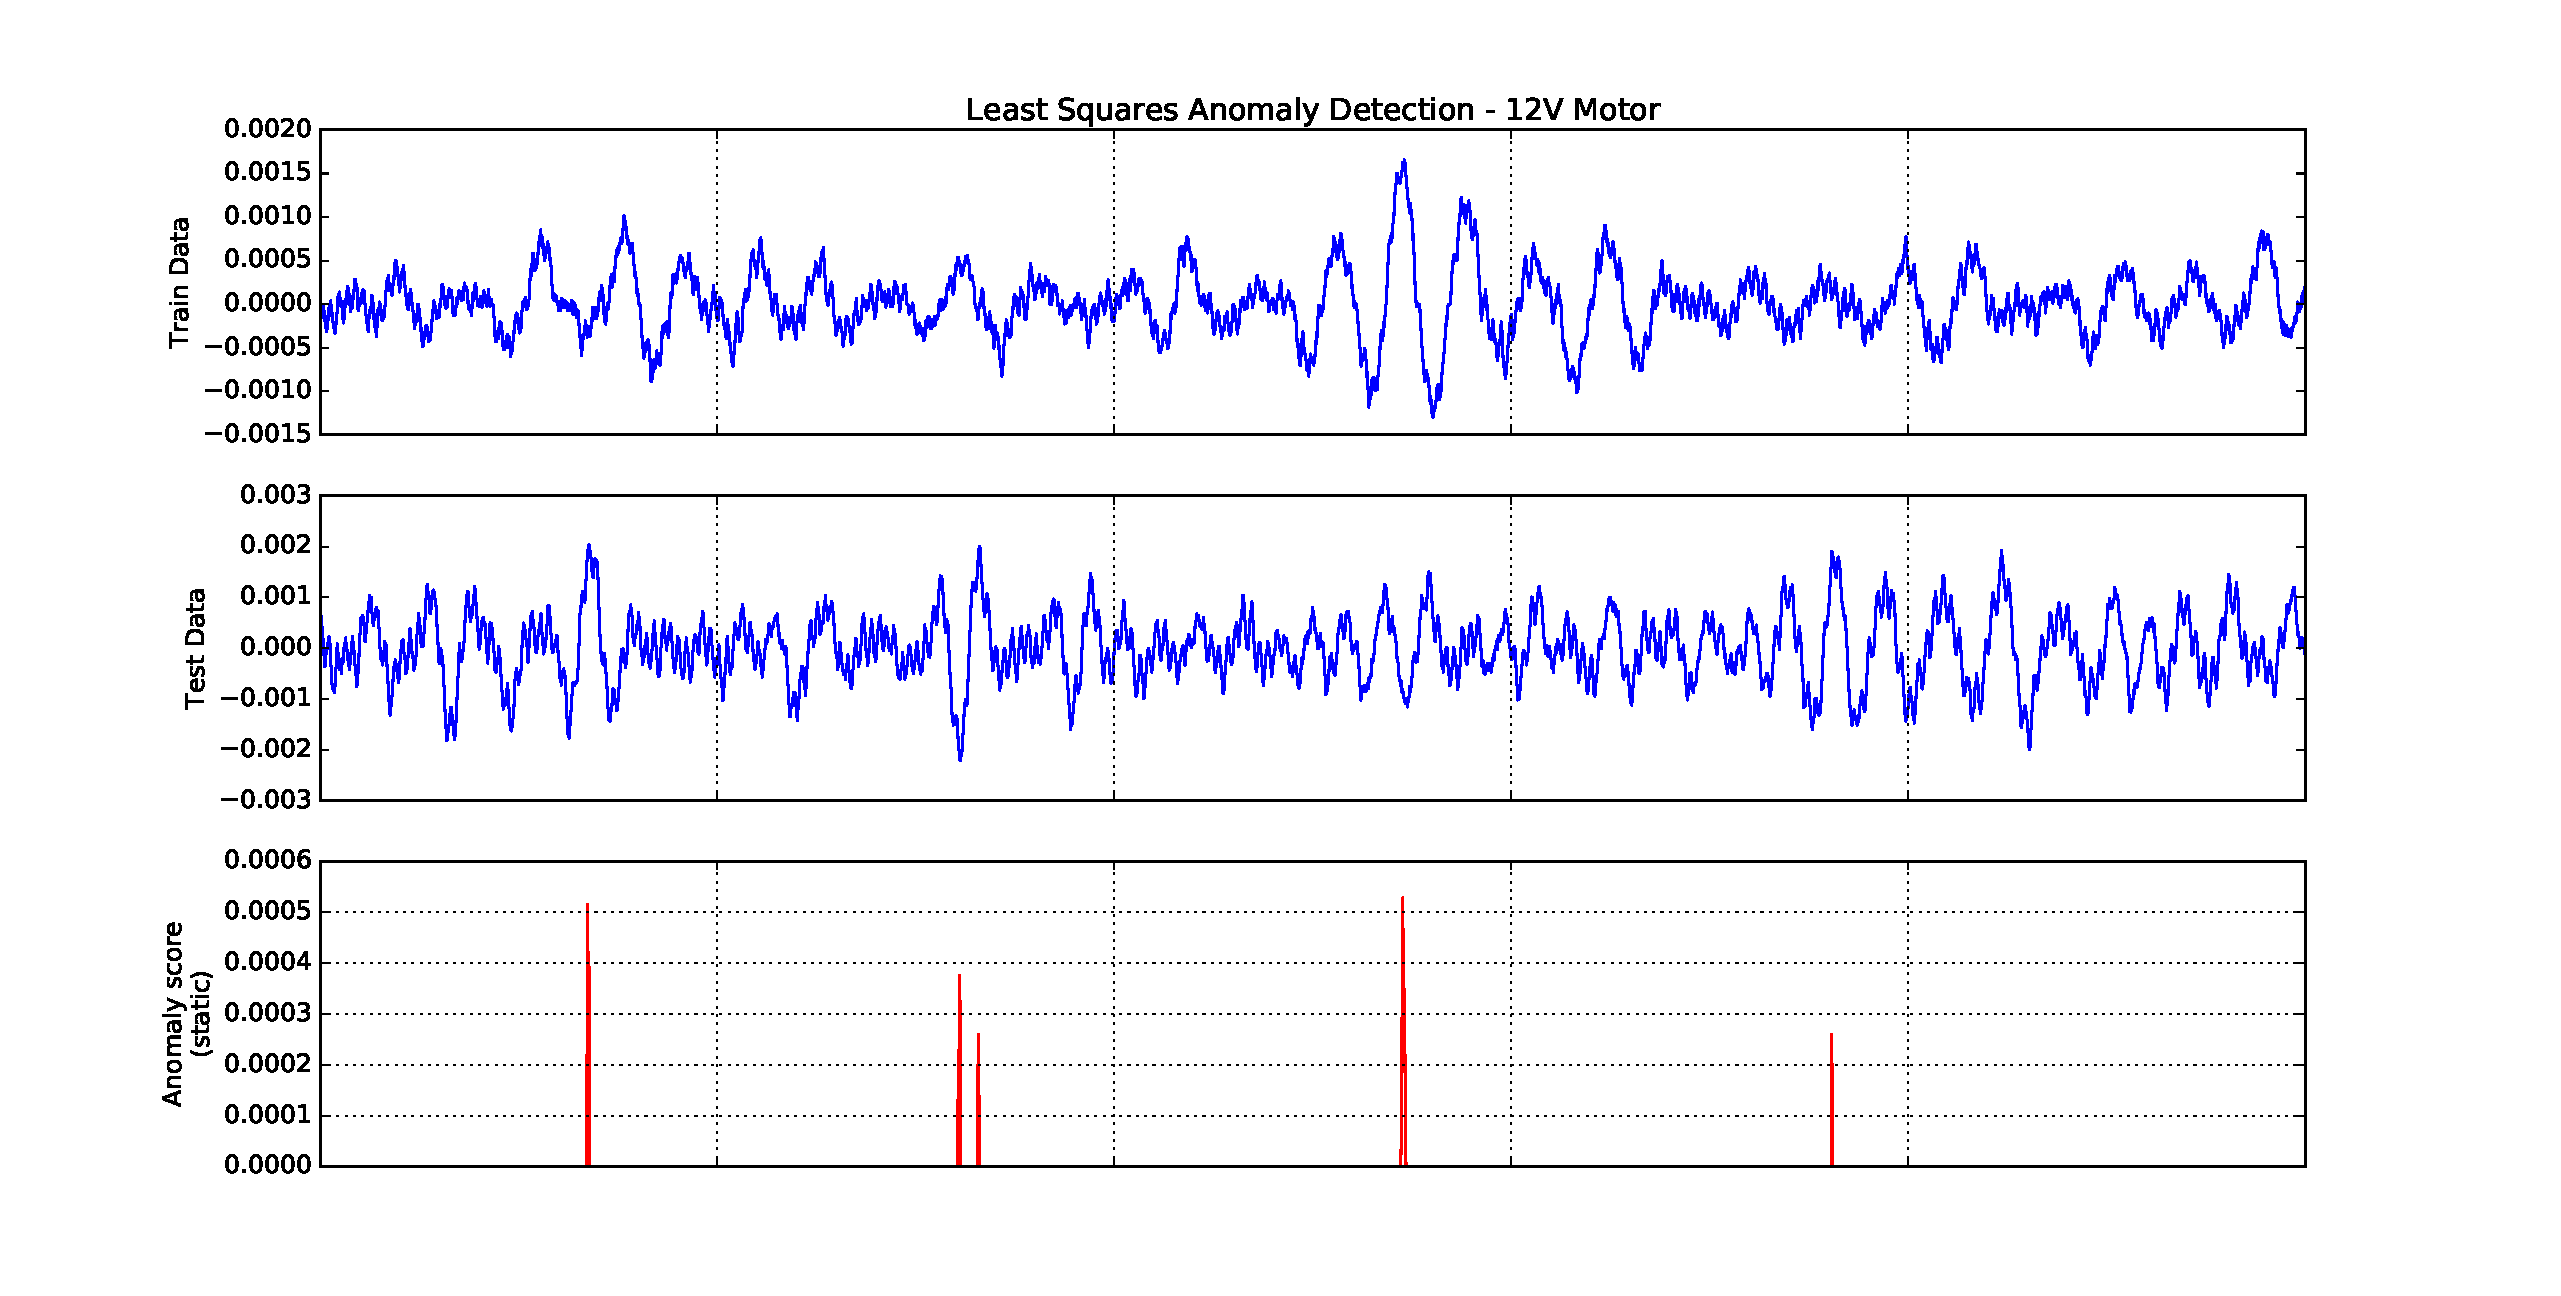
\includegraphics[width=1.0\textwidth]{fig/lsanomaly.pdf}
    \caption[Least Squares Anomaly Score]{Spruced up plot here.}
    \label{fig:lsanomaly}
\end{figure}

\subsection{Machine Learning}  

\subsubsection{K-Means Clustering}
\label{subsec:kmeans}

Cluster analysis involves combining data points into groups, or clusters, in such a way that the points in each cluster are more similar to each other than other points outside of the cluster. Any data points that do not belong to a cluster are defined as outliers. 

Figure~\ref{fig:anomalies} in \S \ref{sec:introduction} shows an example of clusters in 2 dimensions. 

K-means clustering is one of the most highly used cluster analysis methods, due to it being much less computationally intensive in comparison to other approaches \cite{Kanungo:2002:EKC:628329.628801}.

The process involves partitioning a set of n-dimensional data points, of length $N$ ($\{\underline{x}_j\}$ for $j=1,2,...,N$) into a group of $k$ clusters, where $k$ has to be specified by the user. K-means aims to find the centroids $\underline{\mu}_i$ (with $i=1...k$), of the clusters that minimise the Euclidean distance from all data points to their respective clusters, $d(\underline{x}, \underline{\mu}_i) = ||\underline{x}-\underline{\mu}_i||^2$. More formally, K-means clustering finds the centroids of $k$ clusters in order to minimise the expression \cite{596afe3f2b5a4ff3b8f4f9793ad2f4ee},

\begin{equation}
    arg\,min_k \sum_{i=1}^{k} \sum_{\underline{x} \epsilon c_i} ||\underline{x}-\underline{\mu}_i||^2 ~,
    \label{eq:K-means}
\end{equation}

where $c_i$ are the points closest to the cluster $i$.

The general process is described as follows:
\begin{enumerate}
    \item Initialise the centre of the $k$ clusters randomly in Euclidean n-space.
    \item Attribute each data point to the closest cluster centre for that data point. 
    \item Assign a new position for the cluster centre, now given by the barycentre of the data points belonging to the cluster.
    \item Repeat steps 2 and 3 until convergence to a solution is achieved.
\end{enumerate}

Figure~\ref{fig:anomalies} in \S \ref{sec:introduction} shows an example of clusters in 2 dimensions. 

In order to apply K-means clustering to time series data, the n-dimensional space in which the clusters are defined first had to be defined. 

The entire waveform was split into segments in time, with each segment consisting of 12 data points. These segments will then be defined by a set of features, which will form the n-dimensional space. For example, the features could be the mean value and standard deviation of each segment, in which case a 2-dimensional space would be considered. 


The aim is to reconstruct the entire signal using synthetic waveform segments of length 12 data points, which are created from the centroids of the clusters defined in 12-dimensional space. 

Talk about semi-supervised K-means and why this method is semi-supervised rather than unsupervised \cite{596afe3f2b5a4ff3b8f4f9793ad2f4ee}.

\begin{figure}[t]
    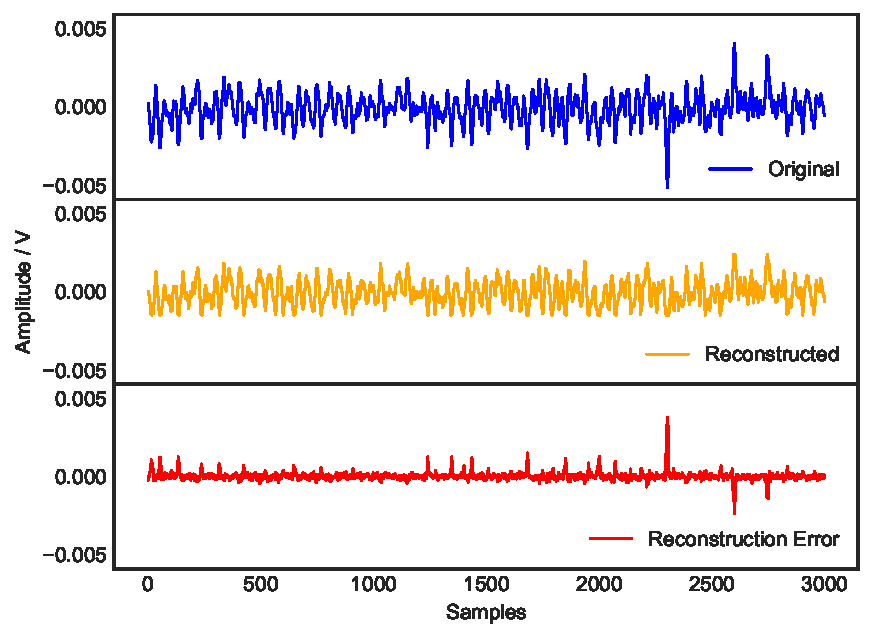
\includegraphics[width=1.0\textwidth]{fig/kmeans.pdf}
    \caption[K mean clustering plot]{Fancy figure goes here.}
    \label{fig:kmeanerror}
\end{figure}

\subsubsection{LSTM Recurrent Neural Networks}
\label{subsec:LSTM}

%Machine learning is the science of programming computers in a manner that means they carry out tasks while not being explicitly programmed. In the past decade, machine learning has given us self-driving cars, practical speech recognition, effective web search, and a vastly improved understanding of the human genome.

Artificial neural networks (ANNs) are a biologically-inspired paradigm that provide a powerful set of techniques that provide solutions to many modern-day problems. In an age of rapidly increasing computational power from graphic processing units, ANNs are rapidly increasing in popularity.

ANNs are best described as a computing system made of many simplistic but highly interconnected layers, which process information by their dynamic state response to an external input. They are `connectionist machines' that simulate the densely interconnected cells that are found in a brain.

A form of ANN known as a recurrent neural network (RNN) consists of a structure of hundreds of thousands of units arranged in layers, which connect to other layers on either side. Some of these units are known as input units - with their role being to receive an information input that the network will attempt to learn about and process. Other types of unit on the other side of the network attempt to form a response to a learned input; these are known as output cells. In between the input and output units are hidden units, which make up the vast majority of the network. Similar to the manner in which neurons in a real brain operate, the links between separate units are assigned weights, in which a positive weight excites the connected unit, and a negative weight suppresses and inhibits the other unit.

RNNs operate by taking an input of information via the input units, triggering layers of hidden units before ending up at the output units. Each unit receives an input from the units that are located earlier in the network. These inputs are multiplied by the weights associated with the connections. The training process for a RNN typically involves the use of a feedback mechanism that propagates the network error backwards through the system.

%HOW THEY LEARN HOW THEY BACKPROPAGATE. WHAT MAKES A RECURRENT

Typical RNNs employ backpropagation training alongside stochastic gradient descent optimisation methods. The combination of these is known as a `backpropagation through time' algorithm. 

What this method involves is an input being passed forward through the neural network, layer by layer, until it reaches the output layer. The network's output is compared to the targeted output with the use of a loss function. An error value is then assigned to each of the `neurons' in the output layer. These error values are then passed backwards through the network, until each layer has an error associated with it that is proportional, and therefore representative of its contribution, to the original output \cite{Graves2012}. The effect of this process is to reduce the difference between the actual and intended output, by modifying the weights of the connections throughout the network. This means the network will be able to `figure something out' from an input, based on how the network has been trained beforehand.

However one problem with RNNs is that the error signal suffers from an exponential decay as it propagates through the network. This means that the front layers train very slowly, with the overall effect being that recurrent neural networks fail to learn in the presence of long lags in time between an input and target events. This problem was formalised by researchers and is known as the `vanishing gradient problem' \cite{hochreiter1991untersuchungen, hochreiter2001gradient}. By the mid-1990s the vanishing gradient problem had emerged as a major obstacle in the performance of recurrent neural networks.

LSTM (long short-term memory) is a type of RNN that was first proposed by \cite{Hochreiter:1997:LSM:1246443.1246450} as a way to overcome the vanishing gradient problem. An LSTM network is extremely well suited for learning tasks such as speech recognition \cite{Graves2005602}, handwriting recognition \cite{graves2008unconstrained} and music composition \cite{eck2002learning}. The properties of LSTM networks also make them extremely valuable for the prediction of time series \cite{gers2001applying}.


%An LSTM cell consists of three gates. The input, forget and output. as well as the cell state. the cell state is like a a conveyor belt. just lets memory flow across unchanged. except for a few minor linear interactions these interactions are the gates. we can add or remove memory from the cell state regulated by that. the optionally let memory through. each is is a sigmoid neural network and a multiplication operation the sigmoid function outputs a values between 0 and 1 which describes how much of each component should be let through we represent each of the following gates through the following equation.

\begin{figure}[t]
    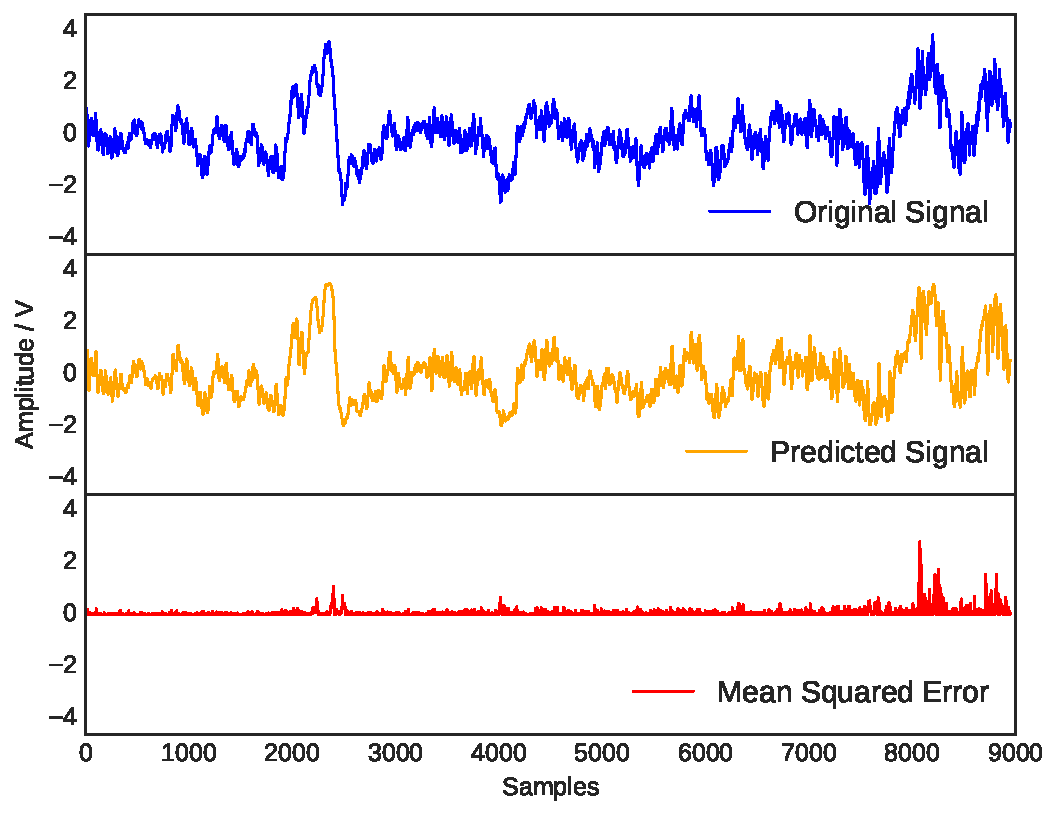
\includegraphics[width=1.0\textwidth]{fig/neuralnetwork.pdf}
    \caption[Neural Network]{Using the LSTM functionality provided by \texttt{Keras}.}
    \label{fig:kmeanerror}
\end{figure}


\subsection{Rejected Methods of Anomaly Detection}
This subsection will include the methods considered for anomaly detection and why they were ultimately rejected to show that a wide range were considered but only certain few were used to ensure quality in the analysis.
 %PROGRAMMERS
\section{Analysis of Motor Data}
\label{sec:analysis}

\subsection{Motor components and setup}

A basic DC motor consists of a stator, a rotor, a commutator, an external magnetic field, brushes, bearings and a shaft. A DC power supply is connected across the brushes, transmitting power through the commutator into windings around the rotor. The current flowing through the windings interacts with the permanent magnetic field producing a Lorentz force, seen in Equation~\eqref{Lorentz} resulting in a torque across the windings.
%reference lorentz
\begin{equation}
    F = I L \times B
    \label{Lorentz}
\end{equation}

As the rotor spins away from a position with the windings perpendicular to the magnetic field, the torque is reduced. To allow a rotational force over the full revolution, commutators invert the current flow periodically. 

\begin{figure}
    \centering
    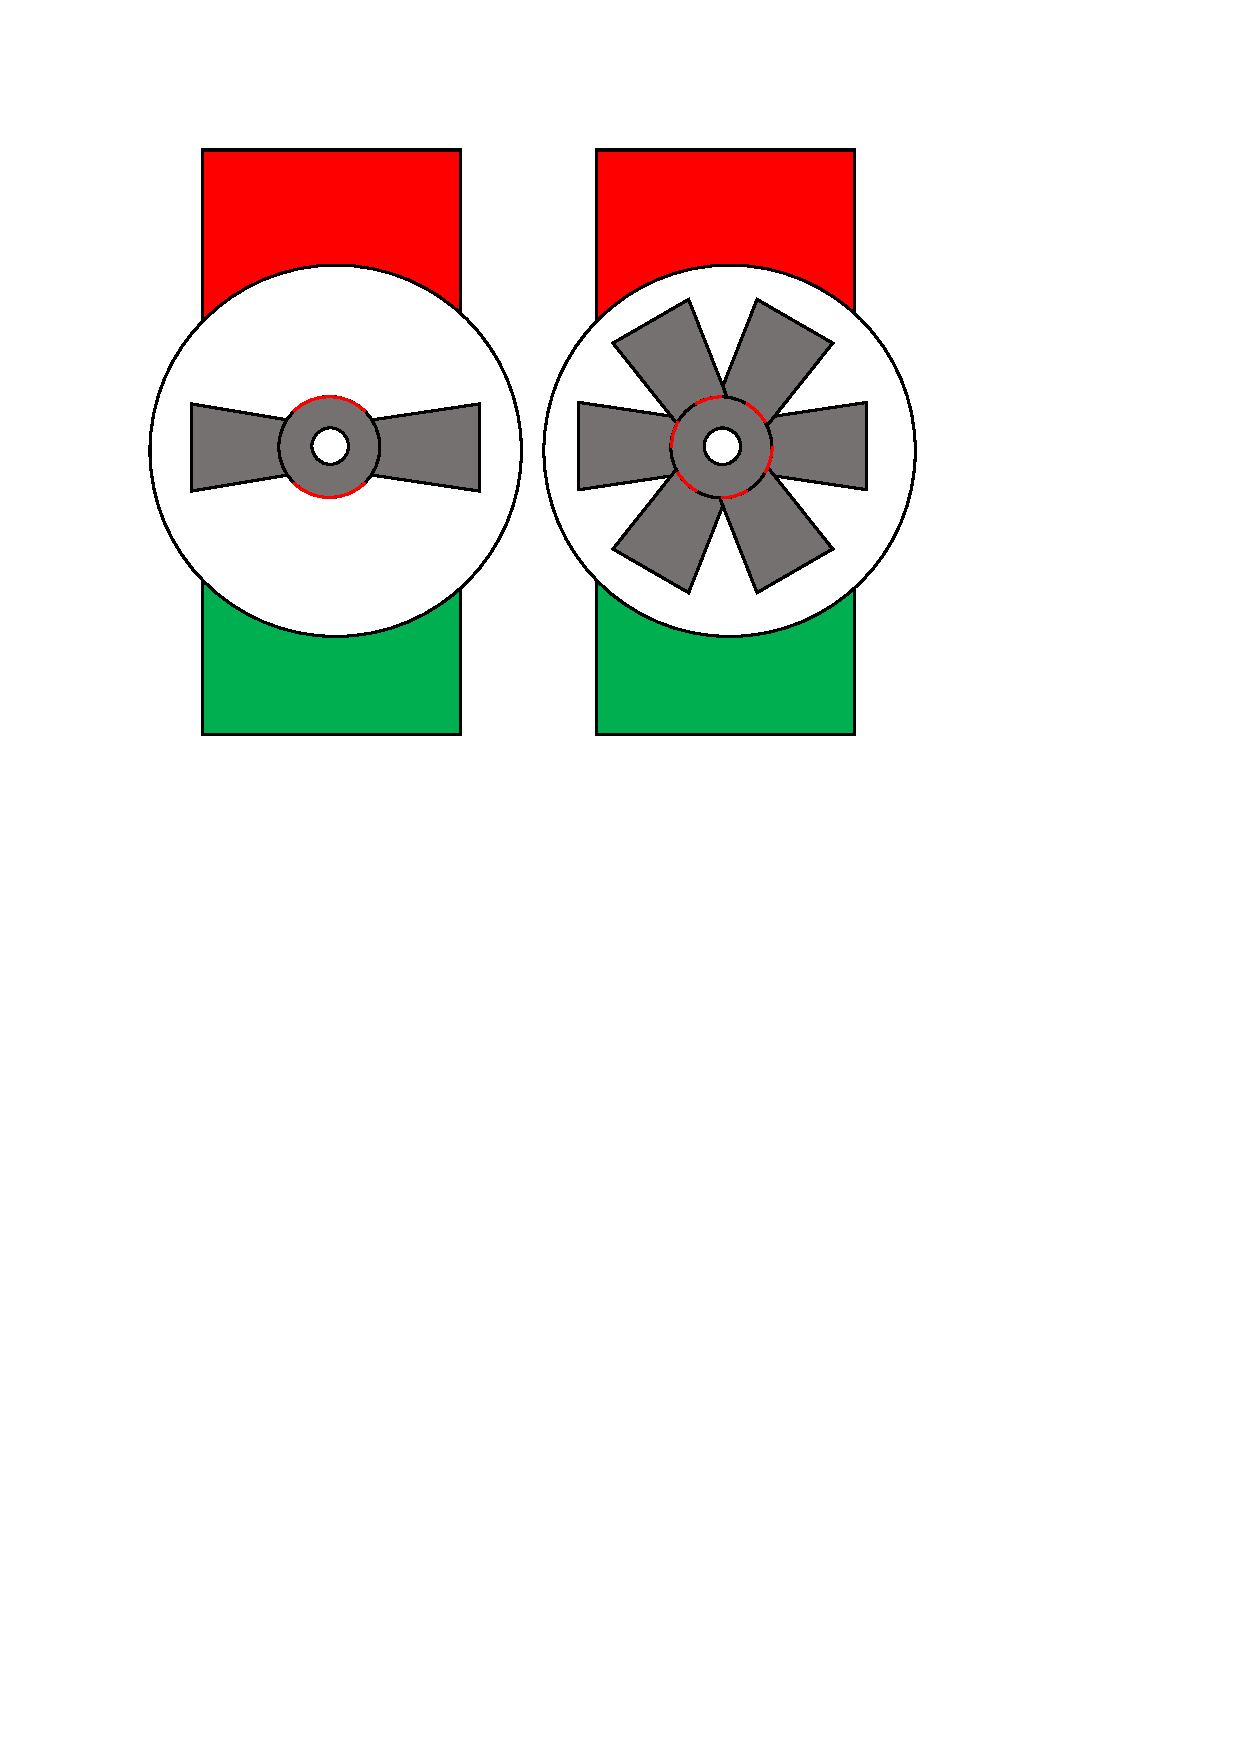
\includegraphics[trim={2cm 15.5cm 0cm 2.548cm}, clip, width=0.8\textwidth]{2polevs6polemotor.pdf}
    \caption[DC motor cross sectional comparison]{This shows a cross sectional comparison between a two pole and six pole motor at various rotation stages. The top left image is labelled showing the: 1. Axle, 2. Commutator, 3. Rotor with windings, 4. Permanent magnets, 5. Stator.}
    \label{fig:2pole_vs_6pole}
\end{figure}

In the simplest possible motor, the rotor is composed of only one set of windings, with a split ring commutator inverting the power supply every half rotation. A more efficient model is to have multiple windings that receive power throughout different stages in the rotation shown in Figure.~\ref{fig:2pole_vs_6pole}. 

At the beginning of the cycle of the two pole motor, the permanent magnetic field is perpendicular to the windings, giving a maximum torque. After one quarter rotation, the windings are parallel to the field. This provides no torque and there is a momentary loss in power as the current is inverted by the commutator. The motor continues to spin due to the momentum gained in the initial stage of rotation until the current is inverted, when torque is regained. For the six pole motor, there is initially a maximum torque supplied by the red marked windings, which decreases to zero at the quarter rotation stage. Unlike the two pole motor, this loss of torque is compensated for, by an increase in torque of the two yellow windings. The torque provided here is more constant than the simple two pole motor, however still not perfectly continuous. An increase in the number of poles increases the continuity of rotation.

The brushes of a motor can be either spring loaded carbon rods, or copper strips pressed against the commutator. Carbon rods are far more efficient and less damaging to the motor, the reasons for this will be discussed further. With advancements in technology, brushless DC motors are becoming increasingly popular, removing the inefficiencies induced by the traditional brushes. 

Mechanical components, such as the bearings, shaft or motor housing are prone to physical damage. This could be due to either physical trauma or a contamination within the motor during operation. Failure of this type would need heavy repairs, with sometimes expensive replacements necessary, it is therefore important to diagnose any unhealthy running motor to minimise the damage.

\begin{figure}
    \centering
    \begin{circuitikz} 
    \draw (0.9,0.75) node[left] {5 V};
    \draw (5.5,0) node[left] {2};
    \draw (5.5,1) node[left] {1};
    \draw (5.5,-1) node[left] {3};
    \draw (10.5,0) node[left] {V$_2$ out};
    \draw (10.5,1) node[left] {V$_1$ out};
    \draw (10.5,-1) node[left] {V$_3$ out};
    \draw
    (0,0) to[battery]  (1,0)
          to[generic]  (9,0) -- (9,0)
          to[short,-o] (9,0)
    ;
    \draw
    (2,0) to[ground] (2,1)
          to[generic] (8,1) -- (8,1)
              to[short,-o] (9,1)
    ;
    \draw
    (2,0) to[ground] (2,-1)
          to[generic] (8,-1) -- (8,-1)
          to[short,-o] (9,-1)
    ;
    \draw
    (8,1) to[short] node[ground] {} (8,-3)
    ;
    \end{circuitikz}
    \caption[Sensor circuit board]{The circuit required to convert data recorded by the contact microphones from an anologue output to digital so that it can accessed by the National instruments DAQ box.}
    \label{fig:circuit_diagram}
\end{figure}

The vibrational data collected by the contact microphones provided an analogue output, which when passed through a NI multifunction DAQ\footnote{NI USB-6009  Multifunction DAQ USB Device, Datasheet: \url{http://www.ni.com/datasheet/pdf/en/ds-218}}, could be converted and saved as a csv file. The circuit diagram showing the configuration of components is displayed in Figure.~\ref{fig:circuit_diagram}. This was produced using a Veroboard.

The rotation speed of a motors shaft can provide a lot of information about the running health of a motor. Measurements of rotation speed can be obtained through the use of a rotary encoder (footnote style thing here) (maybe picture here? Take on Wednesday) which is fitted to the rotating shaft. The encoder is a composed of a codewheel and an emitter/detector module. As the disk spins, the apertures periodically block or allow the light to pass from the emitter to detector, converting the rotary shaft motion into a digital output. The rotary disk has three sections for varying level of accuracy, one channel outputs once per revolution, the other providing higher resolution with COUNT ROTARY ENCODER SLITS.

The quadrature output of the rotary encoder allows monitoring of the shaft rotation speed with time, allowing investigation into certain failure modes such as slipping. This piece of equipment is relatively invasive compared to the contact microphones, as it requires fixing to the shaft, limiting space for operational output. 


\subsection{Calibration Tests}

In order to determine which frequency components were from the motors and what was simply noise (unwanted signal), calibration tests were run for each motor. This involved recording data whilst the motor was off. 

\begin{figure}[t]
    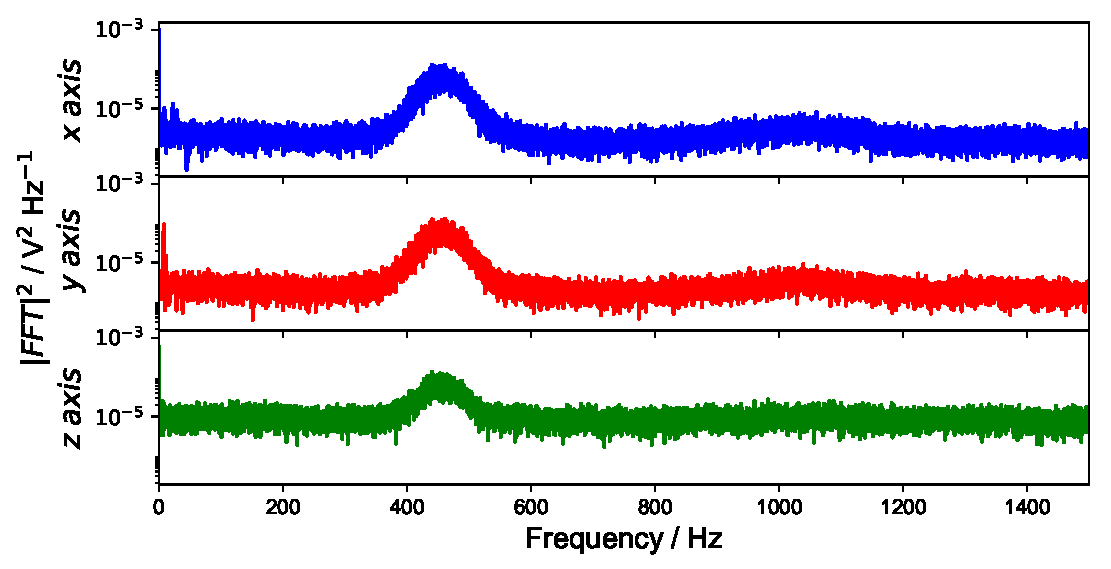
\includegraphics[width=1.0\textwidth]{fig/freq_large_0V.pdf}
    \caption[Calibration Frequency 1]{The Fourier spectra in the x, y, and z axes for the large motor at 0V.}
    \label{fig:freq_large0V}
\end{figure}

Figure~\ref{fig:freq_large0V} shows the frequency spectra for a calibration test with the large motor. 

----write more

\subsection{Baseline Tests}

\begin{figure}[t]
    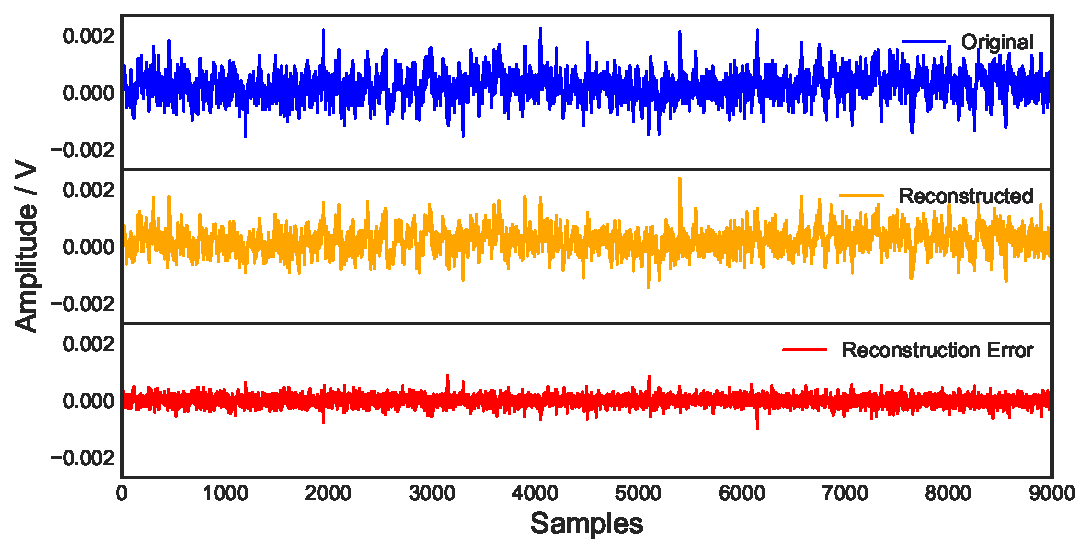
\includegraphics[width=1.0\textwidth]{fig/kmeans_large_4Vnowater.pdf}
    \caption[K-means Large Motor Reconstruction No Water]{K-means reconstruction applied to three seconds of data from large motor running at 4 V. Top: the original testing data. Middle: the reconstruction using K-means. Bottom: the reconstruction error between the reconstructed and original signal.}
    \label{fig:kmeans_large4V}
\end{figure}

Figure.~\ref{fig:kmeans_large4V} shows the K-means reconstruction of a three second signal using training and testing data both from a baseline test run. The first three seconds of the baseline test run was used as training data and the second three seconds used as fitting data. This was done to check if the synthetic segments could be used to recreate a later section of the same baseline run with minimal reconstruction error. 

\subsection{Overheating}
%talk about snipped coils too to simulate each coil breaking separetly.

Overheating is widely regarded as the most common cause of motor failures, with many other types of motor deterioration leading to overheating. This is such a substantial problem that a rise of just 10 $^o$C above the regular running temperature causes the life expectancy of the motor to halve. The life span is halved once again for every 10 $^o$C the temperature is raised further.

The problem arises as, during overheating, the varnish covering the metal wires begins to melt. If this occurs at two points of wires that are in contact, the coil of the motor can short circuit.

%(Gears Removed motor)

In order to induce motor failure, a motor, shown in Figure.~\ref{fig:hotplate_motor}, consisting of 7 coils separately providing power was placed on a hotplate, heated to 150 $^o$C, for one hour. This was compared to the assumed usual running temperature of 60 $^o$C, meaning that just one hour on the hot plate equated to 512 hours of regular use.

For this failure mode, only coil was in direct contact with the plate so as only to damage that coil, leaving the others, ideally, with little impairment. Despite the fact that some heat would obviously be conducted through the motor, the effect of this was considered to be minimal with respect to the effect on the targeted coil.

The result of just one coil being broken is that there would be a brief loss of power in the motor when this coil was in contact with the brushes. Therefore the speed of revolution would no longer be uniform. This can cause other problems to occur in the motor such as damage to the bearings. 

In case this did not result in the targeted coil breaking entirely, a further experiment was devised that simulated this effect. To inhibit just one coil, one of the coils was cut. It was then observed that the rotation speed was not constant with no power being given to the motor for $({2}/{7})$ of the time - due to the fact that either of the two brushes could be in contact with the broken coil. Further coils were cut and the speed noted to become even more erratic until. Once four had been broken, the motor was unable to run at all as there was never a point where two brushes were in contact with working coils.

\begin{figure}[t]
    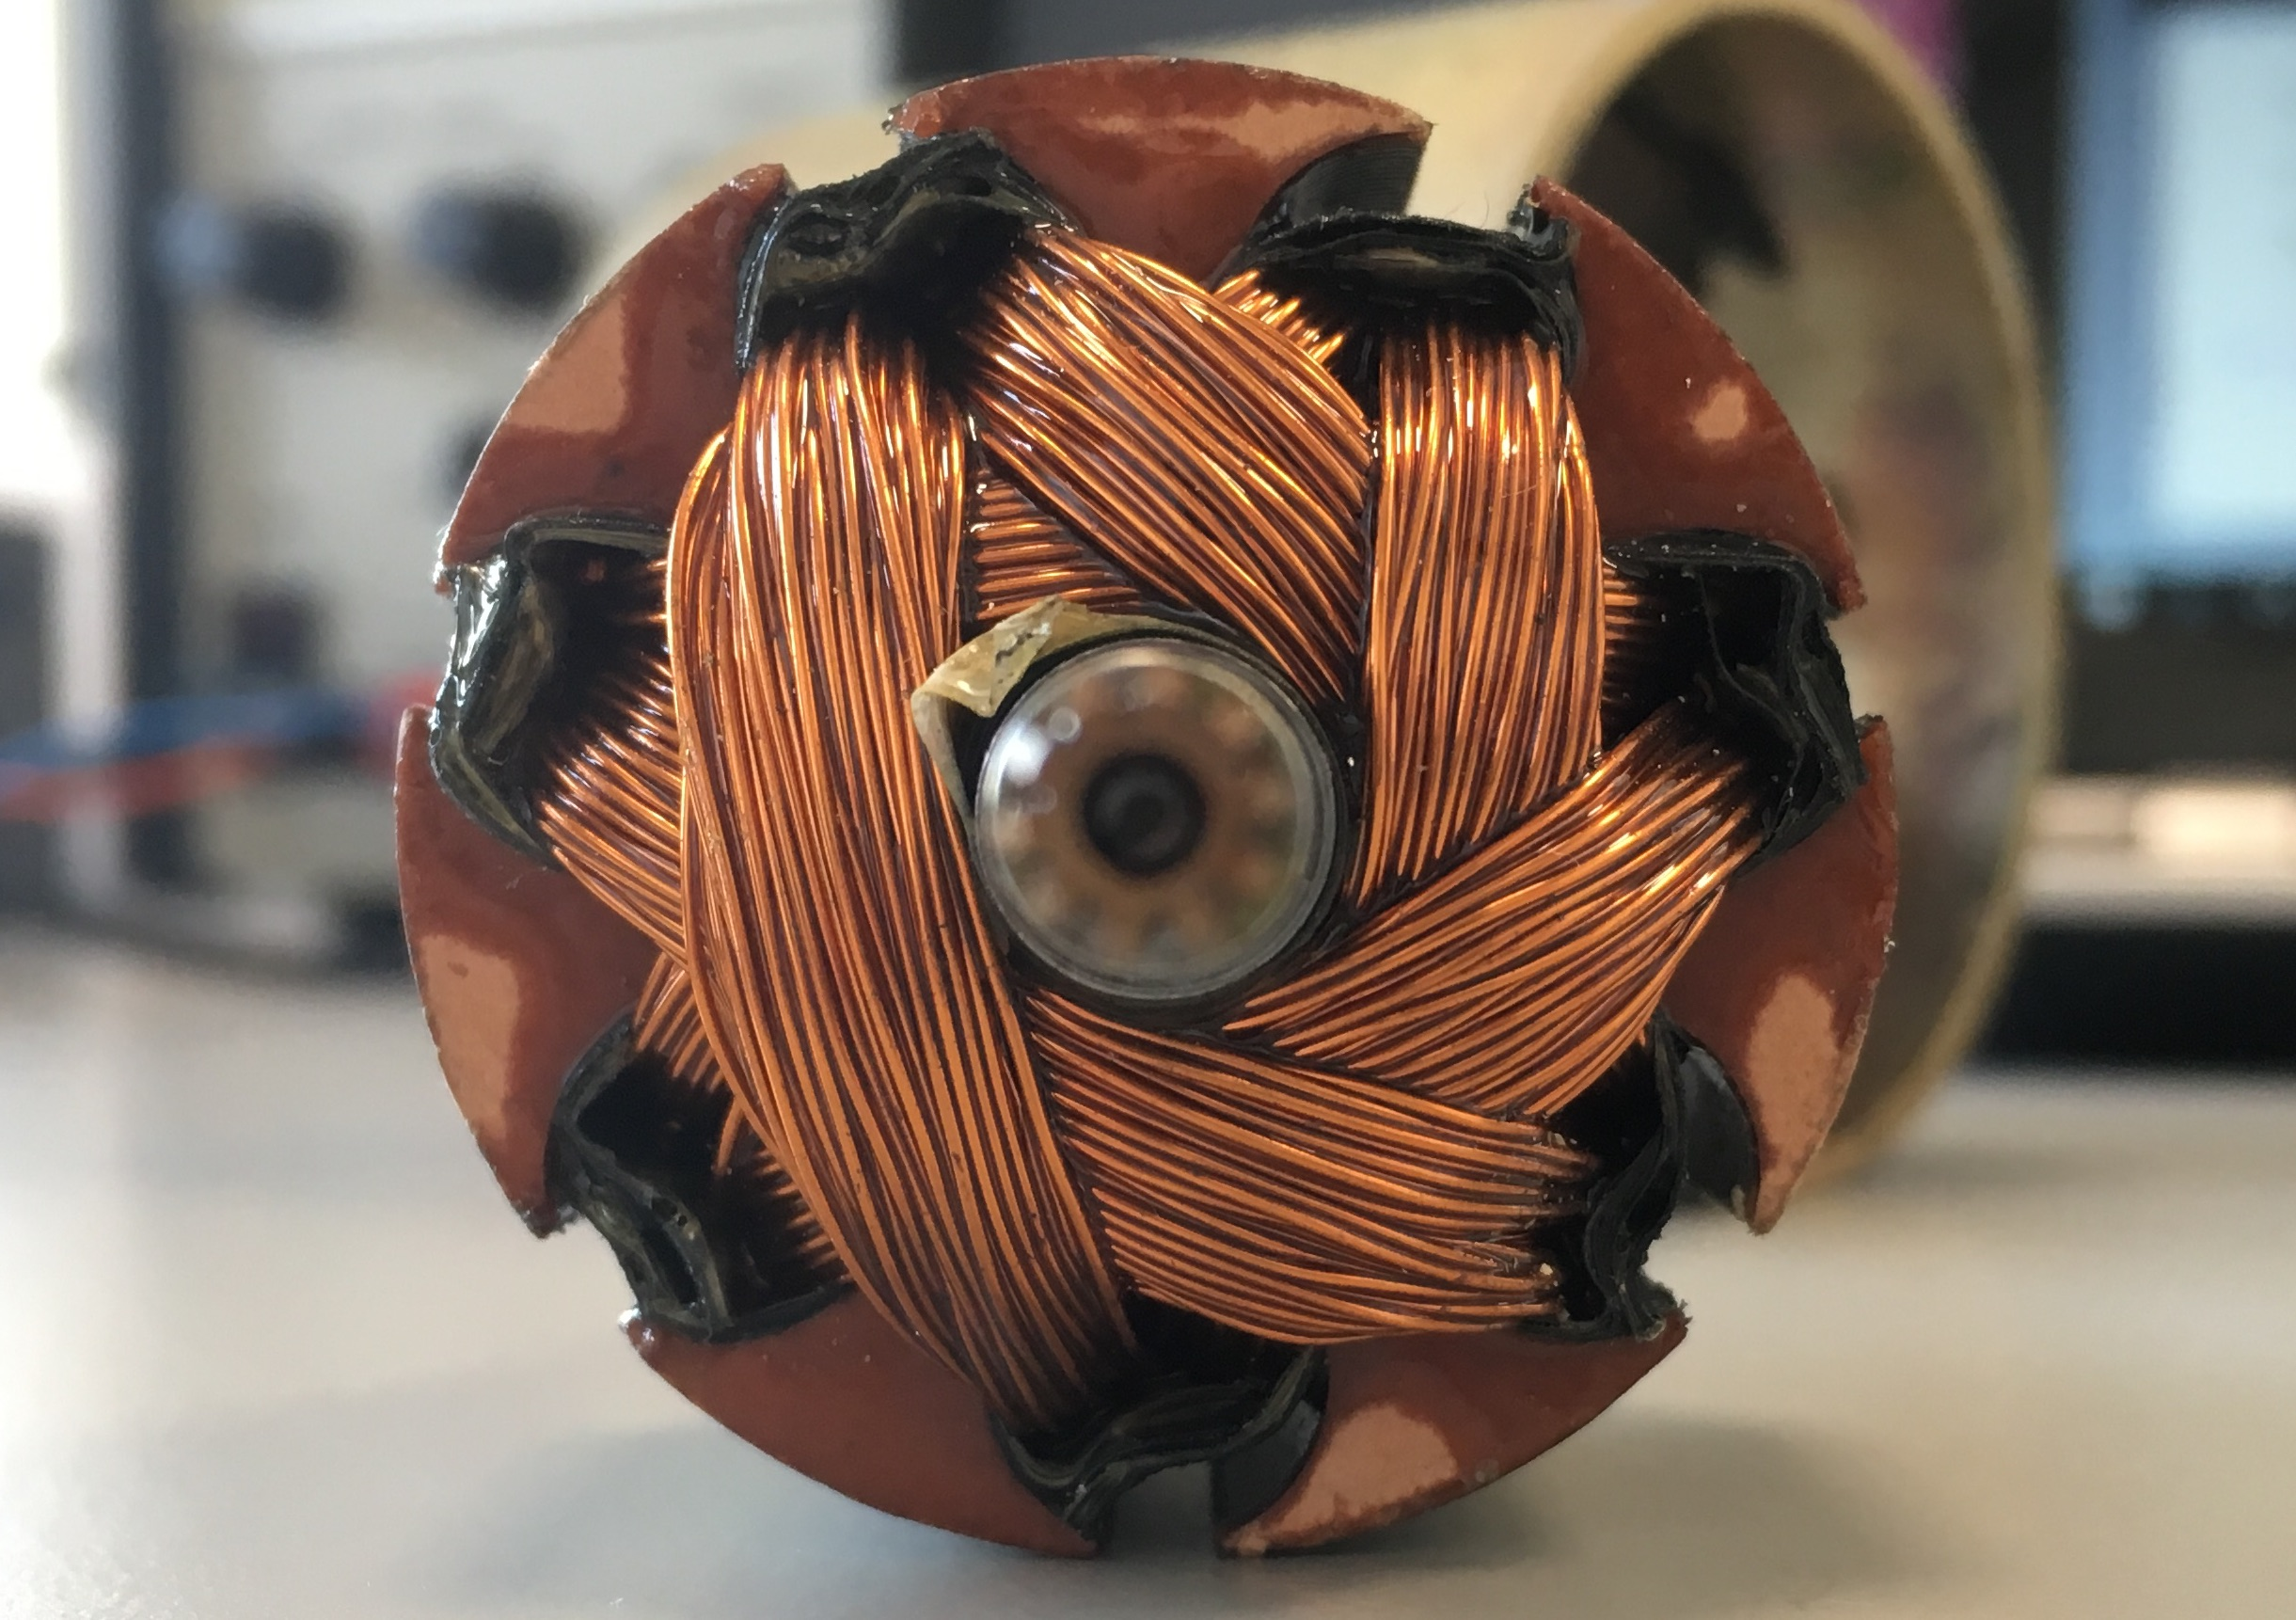
\includegraphics[width=1.0\textwidth]{fig/Gears_Removed_Inside.JPG}
    \caption[Motor Placed on Hotplate]{The inside of the Gears removed motor showing the 7 separate coils, one of which was placed directly on the hotplate at 150 $^o$C for one hour to induce failure.}
    \label{fig:hotplate_motor}
\end{figure}

In addition to this, the motor was placed in an oven at 200 $^o$C for 2 hours to cause extensive damage to all the coils evenly. This equates to over 30,000 hours of running in regular conditions. This was considered sufficient to bring the motor very close to failure given the typical life span of a 12 V motor is just 1000 hours. %1000???
Data was then collected for one minute to find any lasting damage.

%Need references from papers for this


\subsection{Overvoltage}

An increase in voltage will also cause an increase in current, resulting in more eddy currents in the wires and subsequently heating the motor. As stated earlier, this is a major reason for motor failures. 

Moreover, overvoltaging causes the torque of the motor to increase. The subsequent increased rotation speed leads to the rotor slipping. In order to reduce this slip, the motor will then draw an even greater current further contributing to the overheating effect. As well as this, a greater rotation speed will increase friction and will wear down bearings and brushes. Just a small increase in voltage can result in a large amount of damage as,

\begin{equation}
\tau \propto V^2,
\label{Torque}
\end{equation}

where $\tau$ is torque and $V$ is voltage.

In addition to the detrimental effect of overvoltaging, undervoltaging can be just as destructive. In fact, the effect of slipping is even more prominent when a motor is not given enough power and leads to more overheating.

%12V motor

The effect of overvoltaging  was investigated by running a 12 V motor at increasingly high voltages ranging from 12 V to 30 V. This was done for just one minute each time and was used to find the immediate effects of overvoltaging a motor.
    
%Large Motor

A second motor, also with a regular operating voltage of 12 V, was run at 30 V for one hour. In this instance, the bearings reached 90 $^o$C; this demonstrates the extreme effects of overvoltaging a motor. Readings could not be taken during this run as the sensors are only able to operate %Need synonym
up to 60 $^o$C. %Correct???
Therefore, readings were taken before and after the one hour run. This allowed us to explore the long term effects of overvoltaging a motor.

%Undervoltage experiment (large motor)

In order to investigate the effects of undervoltaging a motor, data was collected when running a 12 V motor from 1 V through to 5 V, in 1 V instalments. The speed of rotation could be seen to be irregular, providing evidence that the rotor was slipping. This speed was taken using the rotary encoder, mentioned earlier.

%Again need references.

\subsection{Load}

\begin{figure}[t]
    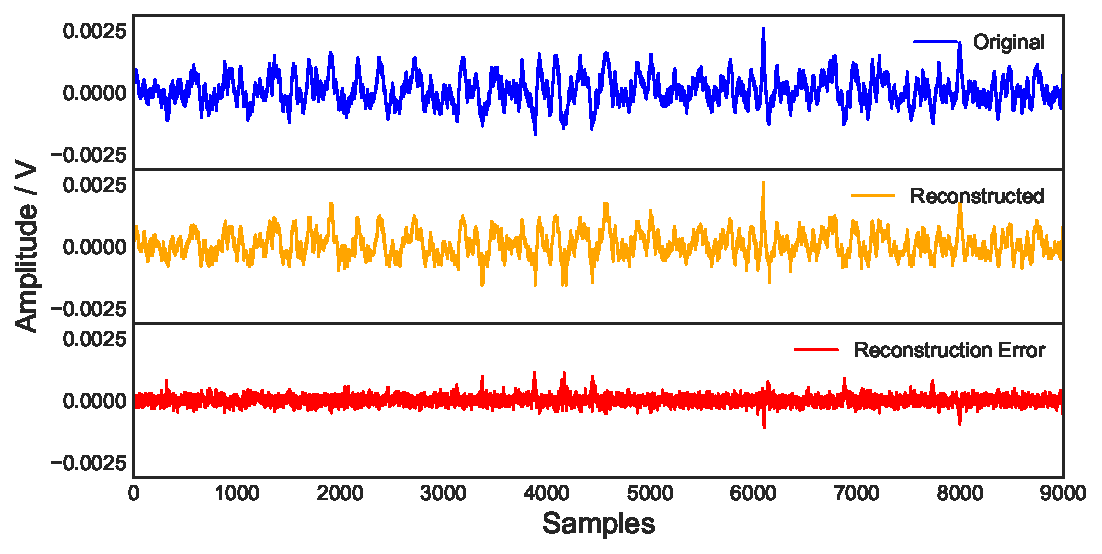
\includegraphics[width=1.0\textwidth]{fig/kmeans_large_4Vwater.pdf}
    \caption[K-means Large Motor Reconstruction In Water]{K-means reconstruction applied to three seconds of data from large motor running at 4V under a load applied through a fan and a bucket of water. Top: the original testing data. Middle: the reconstruction using K-means. Bottom: the reconstruction error between the reconstructed and original signal.}
    \label{fig:kmeans_large4Vwater}
\end{figure}

The presence of a load puts a large amount of stress on the motor. As the motor struggles to reach the desired voltage, a greater current is drawn, which leads to overheating.
        
There are many ways of adding a load to a motor, but attaching a fan immersed in water was chosen due to the ability to vary the load through using fans of different widths (1 cm, 2 cm and 3 cm).
    
Initially the test was done on a 12 V geared motor. A gear ratio of ${5}/{288}$ was found by counting the teeth of each cog and finding the speed of the connecting cog. This meant that the speed of the shaft, $\omega_1$, rotates at a much slower speed than the axle, $\omega _1$ as shown in Equation.~\eqref{eq:gear_Ratio}.

\begin{equation}
\omega_1 = \frac{5}{288} \omega_2.
\label{eq:gear_Ratio}
\end{equation}

This increases the torque of the shaft and resulted in the motor being able to deal with a greater load. It was even able to run at 30 V for the thickest fan.

A test was then conducted for another 12 V motor, this time ungeared. This time the motor could only reach a maximum of 4 V when the 1 cm fan was in use. This is evidence that as a load is added, a greater current is required to achieve a power that is large enough. A 10 A power supply was used for this experiment and this was the limiting factor, preventing the voltage from increasing further.

\subsection{Rotor Imbalance}
As the rotor spins within the motor, it is important for the weight to be evenly distributed around the central axle. Any imbalance present can cause the rotor to shift in position toward the areas of concentrated mass. As a motor runs increased levels of vibrations are produced with the frequency of the vibrations matching the shaft rotation speed. This unnecessarily increases the stress on the bearings and, in extreme cases, this can cause contact between the rotor and the stator. This increased strain on the bearings causes a larger friction, not only reducing the efficiency of the motor but also damaging the bearings. This can lead to complicated maintenance operations that would be otherwise unnecessary for a properly aligned motor.

If there is contact between the rotor and stator, there is again an increase in friction. This is often a larger frictional force, decreasing the efficiency further, but also generating large amounts of heat. When operated in this condition for long periods of time, this can cause overheating discussed above. As the rotor spins against the stator, the friction is capable of causing unwanted damage to both the rotor and the stator. In the case that this force is large enough, the permanent magnets could become detached from the stator, ultimately resulting in a failed motor.

Some possible causes of an imbalanced motor include uneven wear through use, design or assembly errors, and an eccentricity of the rotor or any physical damage distorting components. Observing additional, unexpected frequencies could be due to an imbalance within the motor, and as such are a warning sign to the decline in health of the motor. 

\begin{figure}
    \centering
    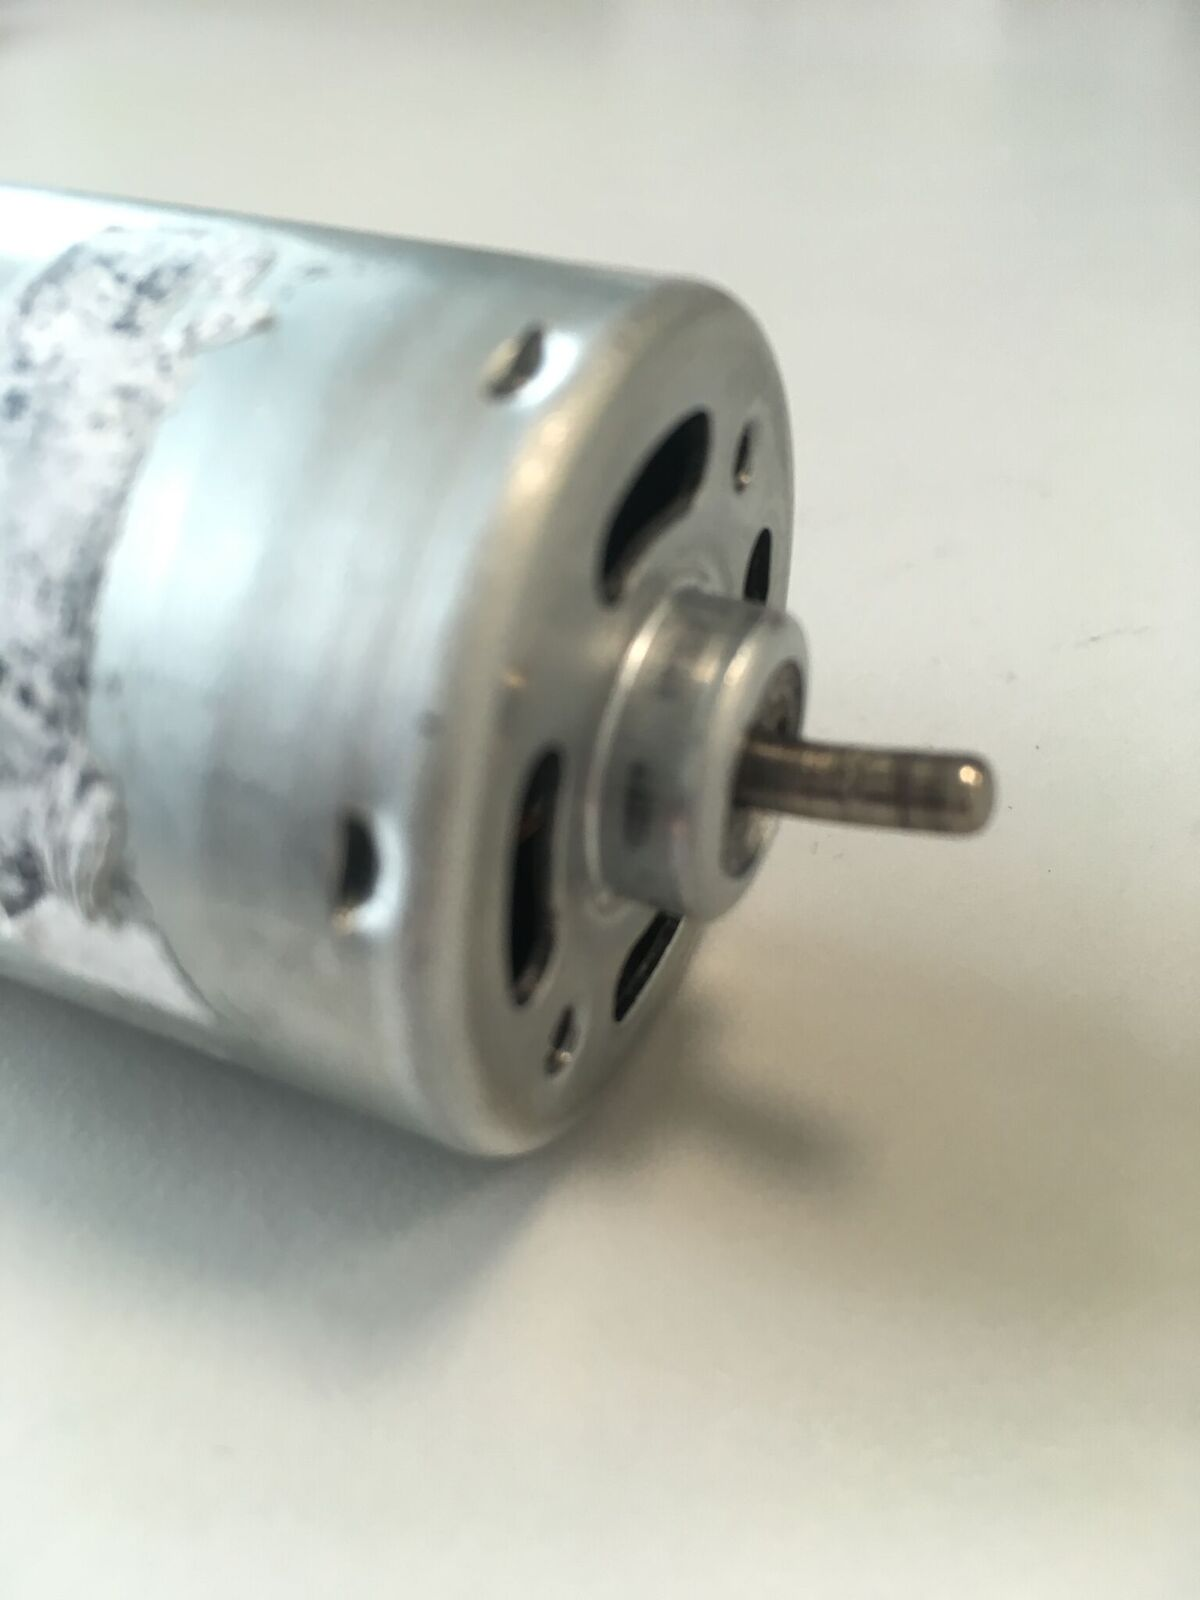
\includegraphics[trim={0cm, 15cm, 0cm, 8cm}, clip, width=0.5\textwidth]{bentshaft1.jpg}
    \caption[Misaligned Motor Shaft]{Small motor with misaligned shaft}
    \label{fig:bentshaft}
\end{figure}

To simulate an imbalanced motor, the shaft of a motor was bent with varying severities. (See Figure.~\ref{fig:bentshaft}.) As with all motors, it is impossible to attain a state of perfect balance, so small bends are expected in any initial baseline test. As the angle of the shaft from the normal was increased, the motors health deteriorated greatly. At large bends, the frictional force became so large that the motor required an initial force to start movement. This could represent a heavy contact between the rotor and the stator. 

%Normally, unbalance will produce a 1x or shaft speed vibration that is 80 percent or more of the total vibration. If 1x vibration is less than 80 percent, suspect other problems in addition to the unbalance.

\subsection{Brush Damage}
The brushes of a DC motor are a vital component, key to the proper working of the motor, allowing a DC power supply to provide an almost constant driving force throughout the entire revolution of the motor. The stationary brushes, combined with the rotating commutator attached to the rotor, periodically inverts the power supply throughout the revolutions. The commutator is composed of strips of conducting metal, usually copper, placed around the rotor. The strips of copper supply the current from the spring loaded brushes to the windings.  Without this periodic inversion of current direction through the windings, the motor would fail to spin and, as such, a good contact between the face of the brush and the commutator is necessary. 

The main cause of damage to the brushes of a DC motor usually occurs during maintenance. The soft surfaces of the carbon brushes can be easily scratched if not handled correctly. It is also possible that dirt can enter the motor housing during operation, which if found between the brush and the commutator, can cause heavy damage. In order to induce this type of failure mode, the brushes were treated with a heavy grit sandpaper, leaving the surface very rough. (picture of rough brushes here). 

It is possible for any imperfections in the surface of the carbon brushes to be removed without intervention during normal operation. As the rotor spins making contact with the face of the brushes, the friction generated is often capable of reducing the magnitude of the scratches. The possibility of this self repair will be investigated. However this friction of the brushes can cause another failure mode, loss of contact due to reduction in size of the brushes over time. This requires the brushes to be entirely replaced, making brushed motors unsuitable for use in remote locations. %more about self repair, what we did, e.g. left running for x volts for y time, more photos

The rough contact between the brush and commutator when damaged can cause sparking, leading to damaged commutators. Replacing the brush on a motor is a relatively simple maintenance task, however replacing the copper strips of a commutator can be more complicated. It is therefore important to ensure that a motor running with damaged brushes is identified immediately, to prevent running in sub-optimal conditions, potentially causing further damage. (picture here of commutator on small 12 V motor, this motor has copper strips for brushes, not carbon, so famously “sparky”)

Due to the flaws in the brushed DC motor model, their use has been declining with the introduction of brushless DC motors. These use an integrated switching power supply, to convert the DC to AC for the motor to run. Another alternative is to simply use an AC motor. 

\subsection{Gear Damage}

%First degreased the gears with a citrus degreasing spray.
%Added dirt to cause gears to break and prevent easy movement.
    %This can lead to overheating
%Placed in water for a few days to cause the motor to rust

\subsection{Specific Failures}

For testing purposed, to ensure that the various anomaly detection algorithms performed as expected, specific anomalies were induced. These included applying a force on the shaft, a routine of taps on the sensors or increasing and decreasing the voltage. The variations in frequencies induced by these actions are not found in a normal working motor, so the algorithm should detect these changes as anomalous. 

\subsection{Soft footing}

A motor running with soft footing can be the cause of multiple failures within a motor. When a motor with a misaligned shaft is coupled with an uneven motor housing, the uneven weight distribution as the rotor spins is exaggerated. The negative impacts of the uneven shaft are amplified, meaning even misalignments can now be damaging. 

The cause of a soft footing can be either an imperfection in the mounting feet of the motor, or the foundations the motor is mounted upon. In either case the motor will have the ability to move in a diagonal plane, similar to a chair or table on uneven ground, causing the shaft to become misaligned. This can be avoided by properly aligning the mountings and the foundations, commonly performed in industry using laser precision tools. 

This failure mode was induced by suspending the large motor above the work surface with a loosely gripped clamp stand. Any movement within the motor could cause a much larger movement in the stand, allowing the motor to oscillate while being suspended in the air. This oscillation will have an impact upon the shaft within the motor, exaggerating movements within the stator. The effects of this are similar to misalignment discussed above. Depending on the frequency of rotation of the motor, a resonance can occur, massively amplifying the oscillations causing an increased level of damage. If the feet do become loose, it is important to be aware of this before long term running of the motor is performed, as this would cause damage to internal components. It is more cost and energy effective to ensure proper footings prior to running.          %JAKE & ROB
\section{Conclusion}
\label{sec:conclusion}

% days of manually constructing features from data are almost over. The machines will win

\subsection{Experimental extensions }

It would be of interest to expand upon the work done overloading an ungeared motor, specifically applying a rotary encoder and an ammeter. This was the initial plan, however the experimental set up rapidly became overcomplicated, meaning it was impractical to take both contact microphone data and rotary encoder data. The revolution speed given by the rotary encoder, coupled with an ammeter in series with the motor, would allow insight into how the speed of the shaft varies with the current drawn and the corresponding vibrations produced. This could reveal more about slipping produced during load application and any momentary losses of power due to this. 






\addcontentsline{toc}{section}{Acknowledgements}
\section*{Acknowledgements}

\small We thank Dr. Chris Saunter, our consultant for this project. We also thank Prof. Paula Chadwick for the Team Project Module. Many thanks to Owen Jones and Carl Tipton from Tracerco who are reponsible for this project idea. We appreciate the help of the Physics department technicians, Paul Foley and Ryan Ellison.




















































\iffalse
We proposed a new algorithm, \emph{EXPoSE}, to perform anomaly detection on very large-scale datasets and streams with concept drift. Although anomaly detection is a problem of central importance in many applications, only a few algorithms are scalable to the vast amount of data we are often confronted with.

The EXPoSE anomaly detection classifier calculates a score (the likelihood of a query point belonging to the class of normal data) using the inner product between a feature map and the kernel embedding of probability measures. The kernel embedding technique provides an efficient way to work with probability measures without the necessity to make assumptions about the underlying distributions.

Despite its simplicity EXPoSE obeys a \emph{linear} computational complexity for learning and can make predictions in \emph{constant} time while it requires only  \emph{constant} memory. 
When applied incrementally or online, a model update can also be performed in \emph{constant} time. We demonstrated that EXPoSE can be used as an efficient anomaly detection algorithm with the same predictive performance as the best state of the art methods while being significant faster than techniques with the same discriminant power.\cite{Habel_2007_IAG}
\fi        %EVERYONE
\clearpage
\hypersetup{%
	colorlinks=true, 
	urlcolor=orange, linkcolor=black, citecolor=blue
}

\addcontentsline{toc}{section}{References}
\bibliographystyle{mnras}
\bibliography{references}
\include{append}
\end{document}




